% =====================================================================
%  Full-Waveform Inversion -- Volume 1: Introdutório (qualitativo)
%  Compile com:  xelatex fwi_nivel1_introdutorio.tex  (duas vezes)
% =====================================================================
\documentclass[11pt,a4paper,oneside]{report}
\usepackage{fwiestilo}

\renewcommand{\nivelnum}{1}
\renewcommand{\nivelnome}{Introdut\'orio}

\begin{document}

\capafwi
{Entender o que a FWI faz, por que funciona\\e por que \'e dif\'icil ---
sem precisar resolver uma integral}
{``A FWI n\~ao tem v\'alvula de escape: o que ela n\~ao consegue explicar
pela f\'isica, ela explica mexendo no modelo.''}
{12 cap\'itulos $\cdot$ mesma espinha dorsal dos tr\^es volumes}

\tableofcontents
\cleardoublepage

% =====================================================================
\chapter*{Como usar esta cole\c{c}\~ao}
\addcontentsline{toc}{chapter}{Como usar esta cole\c{c}\~ao}
\markboth{COMO USAR}{}

Estes s\~ao tr\^es livros que contam \textbf{a mesma hist\'oria} tr\^es vezes,
cada vez com mais profundidade. N\~ao s\~ao tr\^es assuntos diferentes, nem um
resumo seguido de dois aprofundamentos: s\~ao tr\^es passagens completas pela
teoria de Full-Waveform Inversion, com os mesmos doze cap\'itulos, na mesma
ordem, tratando exatamente dos mesmos t\'opicos.

\begin{center}
\begin{tabular}{@{}llp{7.6cm}@{}}
\toprule
\textbf{Volume} & \textbf{N\'ivel} & \textbf{O que muda} \\
\midrule
1 & Introdut\'orio & \emph{O qu\^e} e \emph{por qu\^e}. As ideias, as figuras,
as analogias e as conclus\~oes. As f\'ormulas aparecem, mas s\~ao
\emph{lidas em palavras}, n\~ao derivadas. \\
2 & Intermedi\'ario & \emph{Como se faz}. Todas as dedu\c{c}\~oes completas,
as vers\~oes discretas, os algoritmos, as contas de dimensionamento e os
exerc\'icios. \\
3 & Avan\c{c}ado & \emph{Por que funciona, e quando falha}. Formula\c{c}\~ao
em espa\c{c}os de fun\c{c}\~oes, derivada de Fr\'echet, teoria de
espalhamento, estrutura da Hessiana, invers\~ao multipar\^ametro, funcionais
alternativos e quantifica\c{c}\~ao de incerteza. \\
\bottomrule
\end{tabular}
\end{center}

\section*{A regra que organiza os tr\^es}

\begin{quote}
\textbf{Cap\'itulo $n$ do Volume 1, do Volume 2 e do Volume 3 tratam do mesmo
assunto.} O que cresce \'e a complexidade e a completude, nunca o escopo.
\end{quote}

Isso permite tr\^es modos de leitura, todos leg\'itimos:

\begin{itemize}[leftmargin=*]
\item \textbf{Em profundidade crescente.} Leia o Volume 1 inteiro, depois o 2,
depois o 3. Cada passagem reencontra as mesmas ideias com mais estrutura.
\item \textbf{Por t\'opico.} Est\'a estudando o m\'etodo do estado adjunto?
Leia o Cap\'itulo 6 dos tr\^es volumes em sequ\^encia.
\item \textbf{Por necessidade.} Leia o Volume 2 como texto principal e des\c{c}a
ao 1 quando uma ideia n\~ao fizer sentido, ou suba ao 3 quando precisar do
detalhe fino.
\end{itemize}

Ao longo do texto, marcas como esta apontam o caminho:

\ponte{N\'ivel 2, §6.2}{a dedu\c{c}\~ao completa do gradiente pelo
Lagrangiano, com todos os termos de fronteira.}

\section*{O que este volume espera de voc\^e}

Muito pouco. Voc\^e precisa saber o que \'e uma onda, o que \'e uma derivada,
e ter alguma no\c{c}\~ao de que um computador resolve equa\c{c}\~oes por
aproxima\c{c}\~ao. N\~ao precisa saber geof\'isica, nem c\'alculo variacional,
nem otimiza\c{c}\~ao num\'erica.

\begin{atencao}[Qualitativo n\~ao significa vago]
Este volume evita dedu\c{c}\~oes, n\~ao evita rigor. Toda afirma\c{c}\~ao
aqui \'e verdadeira como escrita, e cada aproxima\c{c}\~ao vem com o nome de
aproxima\c{c}\~ao. Quando uma frase valer apenas sob condi\c{c}\~oes, as
condi\c{c}\~oes est\~ao ditas.

O que voc\^e \emph{n\~ao} vai encontrar aqui \'e a \emph{justificativa}
completa de cada resultado --- essa \'e a fun\c{c}\~ao dos volumes 2 e 3.
\end{atencao}

\section*{Um aviso sobre os n\'umeros}

Os valores num\'ericos, tabelas e figuras fotogr\'aficas desta cole\c{c}\~ao
v\^em do c\'odigo do curso que acompanha o material (diret\'orios
\arq{aulas/} e \arq{fwikit/}), executado e verificado. Onde um n\'umero \'e
apenas ilustrativo --- um exemplo inventado para fixar uma ordem de grandeza
--- o texto diz isso explicitamente. Os desenhos esquem\'aticos s\~ao
esquem\'aticos: servem para mostrar \emph{forma} e \emph{rela\c{c}\~ao}, n\~ao
para ser medidos com r\'egua.

% =====================================================================
\part*{\centering\color{azulfwi} Parte I --- A propaga\c{c}\~ao: o problema direto}
\addcontentsline{toc}{part}{Parte I --- A propaga\c{c}\~ao: o problema direto}

\chapter{O que \'e FWI}
\label{cap:oque}

\begin{ideia}
FWI \'e adivinhar o interior da Terra ajustando um \emph{palpite} at\'e que a
simula\c{c}\~ao do eco produzida por ele fique igual ao eco realmente
gravado --- usando a forma inteira da onda, e n\~ao apenas o instante em que
ela chega.
\end{ideia}

\section{O problema, do jeito mais concreto poss\'ivel}

Imagine um navio arrastando um canh\~ao de ar e um cabo de v\'arios
quil\^ometros com centenas de microfones subaqu\'aticos. A cada poucos
segundos, o canh\~ao dispara. O som desce, atravessa camadas de sedimento,
reflete nas interfaces, volta, e cada microfone grava um tra\c{c}o: uma curva
de press\~ao contra o tempo.

No fim do levantamento existem milhares desses tra\c{c}os. E existe uma
pergunta: \textbf{qual distribui\c{c}\~ao de velocidade do som na
subsuperf\'icie produziria exatamente esses tra\c{c}os?}

\begin{center}
\begin{tikzpicture}[scale=1.0]
% agua
\fill[cianofwi!12] (0,0) rectangle (13,1.5);
% camadas
\fill[amarelofwi!14] (0,-1.2) rectangle (13,0);
\fill[verdefwi!14]  (0,-2.4) rectangle (13,-1.2);
\fill[vermelhofwi!12] (0,-3.2) rectangle (13,-2.4);
\draw[gray!60] (0,0) -- (13,0);
\draw[gray!60] (0,-1.2) -- (13,-1.2);
\draw[gray!60] (0,-2.4) .. controls (5,-2.1) and (9,-2.7) .. (13,-2.4);
\draw[line width=1pt, azulfwi] (0,1.5) -- (13,1.5);
% navio
\fill[azulfwi] (1.1,1.5) -- (2.3,1.5) -- (2.05,1.95) -- (1.35,1.95) -- cycle;
\node[font=\scriptsize, azulfwi] at (1.7,2.25) {navio};
% fonte
\fill[vermelhofwi] (2.0,1.0) circle (0.11);
\node[font=\scriptsize, vermelhofwi, right=1pt] at (2.1,1.05) {fonte};
% receptores
\foreach \x in {3.0,3.8,4.6,5.4,6.2,7.0,7.8,8.6,9.4,10.2,11.0,11.8} {
  \draw[verdefwi, line width=0.8pt] (\x,1.0) -- (\x,1.25);
  \fill[verdefwi] (\x,1.0) circle (0.055);
}
\node[font=\scriptsize, verdefwi] at (8.8,1.78) {receptores (cabo)};
% raios
\draw[vermelhofwi, line width=0.7pt, ->] (2.0,1.0) -- (4.3,-1.2) -- (6.6,1.0);
\draw[vermelhofwi!70, line width=0.7pt, ->] (2.0,1.0) -- (5.6,-2.4) -- (9.2,1.0);
\draw[vermelhofwi!45, line width=0.7pt, ->] (2.0,1.0) -- (2.6,0) -- (3.2,1.0);
% rotulos camadas
\node[font=\scriptsize, gray!70] at (12.2,0.75) {\'agua};
\node[font=\scriptsize, gray!70] at (12.2,-0.6) {$c_1$};
\node[font=\scriptsize, gray!70] at (12.2,-1.8) {$c_2$};
\node[font=\scriptsize, gray!70] at (12.2,-2.9) {$c_3$};
\end{tikzpicture}
\end{center}

Essa \'e a pergunta que a FWI responde. E note desde j\'a a assimetria que
governa tudo: \textbf{\'e f\'acil ir do modelo para o dado, e dif\'icil ir do
dado para o modelo}. Dado um mapa de velocidades, o computador simula a
propaga\c{c}\~ao e produz os tra\c{c}os --- trabalhoso, mas direto. O caminho
inverso n\~ao tem f\'ormula.

\begin{analogia}[A analogia que funciona]
Voc\^e bate na parede e escuta. Pelo som, descobre se atr\'as dela h\'a
tijolo maci\c{c}o, gesso ou vazio. Voc\^e faz isso o tempo todo, e faz
bem --- mas faz por compara\c{c}\~ao com sons que j\'a ouviu.

A FWI faz a mesma coisa sem ter ouvido nada antes. No lugar da mem\'oria, ela
usa um simulador: tenta uma parede, simula o som que ela produziria, compara
com o som gravado, e corrige a parede. Muitas vezes.
\end{analogia}

\begin{matematica}[como se l\^e uma f\'ormula deste tipo]
A f\'ormula da pr\'oxima p\'agina \'e a \'unica que voc\^e precisa
reconhecer neste volume. Tr\^es s\'imbolos, e depois ela fica leg\'ivel.

\textbf{$\norm{\cdot}$, a ``norma''.} \'E o tamanho de uma lista de
n\'umeros: eleve cada um ao quadrado, some tudo, tire a raiz. Se a lista \'e a
discord\^ancia entre simulado e medido, amostra por amostra, ent\~ao a norma
\'e um \'unico n\'umero que resume o erro inteiro.

Por que \emph{ao quadrado}? Por duas raz\~oes. Primeiro, para que erros
positivos e negativos n\~ao se cancelem. Segundo, porque o quadrado \'e
suave --- tem derivada em toda parte ---, e todo o m\'etodo depende de
derivar. O pre\c{c}o \'e que erros grandes pesam \emph{desproporcionalmente}:
um erro 10 vezes maior conta 100 vezes mais.

\textbf{$\min$ contra $\argmin$.} ``$\min$'' devolve o \emph{menor valor};
``$\argmin$'' devolve o \emph{lugar} onde esse menor valor acontece. Numa
paisagem de montanhas: $\min$ \'e a altitude do fundo do vale, $\argmin$ s\~ao
as coordenadas do fundo do vale. \'E o segundo que interessa aqui --- o
modelo.

\textbf{$F(\mvec)$, o ``operador''.} \'E s\'o um nome curto para ``rode a
simula\c{c}\~ao inteira com esse modelo e me devolva os tra\c{c}os''. Escrever
$F$ em vez de descrever o procedimento \'e conveni\^encia de nota\c{c}\~ao,
n\~ao sofistica\c{c}\~ao: por tr\'as de cada $F(\mvec)$ h\'a horas de
computador.
\end{matematica}

\section{A formula\c{c}\~ao em uma linha}

Toda a FWI cabe em uma linha de matem\'atica. Voc\^e n\~ao precisa saber
resolv\^e-la para entend\^e-la:
\begin{equation}
\mvec^{*} = \argmin_{\mvec}\; J(\mvec),
\qquad
J(\mvec) = \tfrac{1}{2}\,\bigl\|\,F(\mvec) - \dobs \,\bigr\|^{2}.
\label{eq:fwi1}
\end{equation}

Leia assim, da direita para a esquerda:

\begin{itemize}[leftmargin=*]
\item $\dobs$ \'e o \textbf{dado observado} --- os tra\c{c}os gravados no
levantamento. \'E um n\'umero enorme de amostras, mas \'e apenas isso: o que
foi medido.
\item $\mvec$ \'e o \textbf{modelo} --- o palpite atual sobre a
subsuperf\'icie. Na vers\~ao mais simples, um mapa de velocidade do som,
ponto a ponto.
\item $F(\mvec)$ \'e a \textbf{modelagem}: simular a propaga\c{c}\~ao da onda
nesse modelo e gravar o que os receptores teriam registrado. \'E o
``dado sint\'etico''.
\item $F(\mvec) - \dobs$ \'e o \textbf{res\'iduo}: a discord\^ancia entre o
simulado e o medido, amostra por amostra.
\item $\norm{\cdot}^{2}$ soma os quadrados de todas essas discord\^ancias, e
$J$ \'e o n\'umero \'unico que resume ``o qu\~ao errado est\'a o meu
palpite''.
\item $\argmin$ diz: procure o modelo que torna esse n\'umero o menor
poss\'ivel.
\end{itemize}

\begin{teoria}[Por que ``\emph{full-waveform}'']
M\'etodos mais antigos --- a tomografia de tempo de tr\^ansito --- usam
apenas \emph{um n\'umero por evento}: o instante em que a onda chegou. Jogam
fora a amplitude, a forma do pulso, e os eventos que n\~ao foram
identificados.

A FWI usa \textbf{a forma de onda inteira}: cada amostra de cada tra\c{c}o
entra na conta. Da\'i vem a resolu\c{c}\~ao muito maior --- e da\'i v\^em
todas as dificuldades, porque agora o simulador precisa acertar a amplitude e
a fase de tudo, n\~ao s\'o o tempo de chegada de alguns eventos escolhidos.
\end{teoria}

\section{O ciclo}

A resolu\c{c}\~ao de \eqref{eq:fwi1} \'e sempre iterativa: melhorar o palpite
aos poucos. O ciclo abaixo \'e a espinha dorsal de todo o resto desta
cole\c{c}\~ao --- cada caixa vira um cap\'itulo.

\begin{center}
\begin{tikzpicture}[scale=1, transform shape,
  node distance=8mm,
  cx/.style={draw, rounded corners=3pt, line width=0.9pt, align=center,
             minimum height=1.0cm, font=\small, inner sep=4pt},
  seta/.style={-{Stealth[length=2.6mm]}, line width=0.9pt, gray!70}]

\node[cx, draw=azulfwi, fill=azulfwi!7, text width=2.5cm] (m0)
  {\textbf{modelo atual}\\[-1pt]{\scriptsize $\mvec_k$}};
\node[cx, draw=cianofwi, fill=cianofwi!7, right=11mm of m0, text width=2.6cm] (sim)
  {\textbf{simula\c{c}\~ao}\\[-1pt]{\scriptsize $F(\mvec_k)$ --- Caps.\ 2--4}};
\node[cx, draw=amarelofwi, fill=amarelofwi!10, right=11mm of sim, text width=2.5cm] (res)
  {\textbf{res\'iduo}\\[-1pt]{\scriptsize $F(\mvec_k)-\dobs$ --- Cap.\ 5}};
\node[cx, draw=roxofwi, fill=roxofwi!7, below=12mm of res, text width=2.6cm] (grad)
  {\textbf{gradiente}\\[-1pt]{\scriptsize estado adjunto --- Cap.\ 6}};
\node[cx, draw=verdefwi, fill=verdefwi!7, below=12mm of sim, text width=2.7cm] (passo)
  {\textbf{passo}\\[-1pt]{\scriptsize otimiza\c{c}\~ao --- Cap.\ 8}};
\node[cx, draw=azulfwi, fill=azulfwi!7, below=12mm of m0, text width=2.5cm] (m1)
  {\textbf{modelo novo}\\[-1pt]{\scriptsize $\mvec_{k+1}$}};

\node[draw=gray!50, dashed, rounded corners=2pt, right=10mm of res,
      text width=1.7cm, align=center, font=\scriptsize, inner sep=3pt] (dobs)
  {dado observado $\dobs$};

\draw[seta] (m0) -- (sim);
\draw[seta] (sim) -- (res);
\draw[seta] (dobs) -- (res);
\draw[seta] (res) -- (grad);
\draw[seta] (grad) -- (passo);
\draw[seta] (passo) -- (m1);
\draw[seta] (m1) -- ++(-1.4,0) |- ($(m0.west)+(-1.4,0)$) -- (m0);
\node[font=\scriptsize, gray!70, left=1mm of m1] {};
\end{tikzpicture}
\end{center}

\section{As tr\^es dificuldades que definem o campo}

A equa\c{c}\~ao \eqref{eq:fwi1} \'e simples de escrever e brutal de resolver,
por tr\^es raz\~oes \emph{independentes}. Toda a literatura de FWI, e todos os
cap\'itulos que v\^em a seguir, existem por causa de uma dessas tr\^es.

\begin{enumerate}[leftmargin=*]
\item \textbf{Simular \'e caro.} Cada avalia\c{c}\~ao de $F$ \'e uma
simula\c{c}\~ao completa da equa\c{c}\~ao da onda, para cada disparo. Em um
levantamento com centenas de disparos e dezenas de itera\c{c}\~oes, isso \'e
o or\c{c}amento inteiro do projeto. Da\'i a Parte I: simular \emph{certo} e
simular \emph{barato} n\~ao s\~ao detalhes t\'ecnicos, s\~ao a
viabilidade.

\item \textbf{Existem muitos vales errados onde cair.} A fun\c{c}\~ao
$J$ tem m\'inimos locais por toda parte, e o algoritmo desce sempre para o
mais pr\'oximo. O fen\^omeno tem nome pr\'oprio --- \emph{cycle skipping} ---
e uma causa f\'isica precisa, que \'e o assunto do Cap\'itulo~\ref{cap:misfit}.

\item \textbf{O modelo \'e gigante.} De dezenas de milhares a centenas de
milh\~oes de inc\'ognitas --- uma por c\'elula da malha. Isso elimina de
sa\'ida qualquer m\'etodo que precise escrever uma matriz do tamanho do
modelo ao quadrado, e elimina o c\'alculo do gradiente por for\c{c}a bruta.
\'E o Cap\'itulo~\ref{cap:adjunto}.
\end{enumerate}

\begin{teoria}[A ideia sem a qual a FWI n\~ao existiria]
Para melhorar o modelo \'e preciso saber, para cada uma das --- digamos ---
um milh\~ao de c\'elulas, se aumentar a velocidade ali faria $J$ subir ou
descer. Isso \'e o \textbf{gradiente}.

O jeito \'obvio de descobrir: mexa numa c\'elula, refa\c{c}a a
simula\c{c}\~ao, veja o que aconteceu com $J$; repita para cada c\'elula.
Custo: um milh\~ao de simula\c{c}\~oes \emph{por itera\c{c}\~ao}.
Inviabiliza tudo.

O \textbf{m\'etodo do estado adjunto} obt\'em o gradiente inteiro com
\textbf{duas} simula\c{c}\~oes por disparo --- uma para a frente e uma para
tr\'as --- e o custo \textbf{n\~ao depende do n\'umero de c\'elulas}. \'E a
diferen\c{c}a entre imposs\'ivel e rotineiro.
\end{teoria}

\section{O que a FWI recupera bem, e o que n\~ao recupera}

Expectativa calibrada evita meses perdidos. A FWI reconstr\'oi bem os
comprimentos de onda \textbf{intermedi\'arios} do modelo. Ela
\emph{n\~ao} reconstr\'oi:

\begin{itemize}[leftmargin=*]
\item \textbf{a tend\^encia regional de velocidade} (os comprimentos de onda
muito longos): o dado s\'ismico n\~ao tem frequ\^encia baixa o suficiente para
restringi-la. Isso tem de vir do modelo inicial;
\item \textbf{o que est\'a abaixo da profundidade de penetra\c{c}\~ao},
controlada pela abertura da aquisi\c{c}\~ao --- regra pr\'atica: entre um
ter\c{c}o e metade do maior afastamento fonte--receptor;
\item \textbf{detalhes menores que cerca de meio comprimento de onda} da maior
frequ\^encia \'util;
\item \textbf{qualquer coisa em zona de sombra}, onde nenhuma onda passou. Ali
o dado n\~ao cont\'em informa\c{c}\~ao, e nenhum algoritmo cria
informa\c{c}\~ao que n\~ao existe.
\end{itemize}

\begin{atencao}[A frase para levar]
A FWI \textbf{melhora} um modelo; ela n\~ao o \textbf{cria}. Um resultado de
FWI deve sempre ser reportado ao lado do modelo do qual ele partiu --- sem
isso, o n\'umero final n\~ao significa nada. Voltamos a esse ponto, com
n\'umeros, no Cap\'itulo~\ref{cap:completa}.
\end{atencao}

\begin{resumo}
\begin{itemize}[leftmargin=*, itemsep=1pt]
\item FWI procura o modelo de subsuperf\'icie cuja \emph{simula\c{c}\~ao} da
onda melhor reproduz o dado gravado, usando a forma de onda inteira.
\item Ir do modelo ao dado \'e direto; o contr\'ario n\~ao tem f\'ormula ---
por isso se resolve iterando.
\item Tr\^es dificuldades independentes organizam o campo: simular \'e caro,
a fun\c{c}\~ao objetivo tem m\'inimos locais, e o modelo \'e grande demais
para for\c{c}a bruta.
\item A FWI recupera bem as escalas intermedi\'arias; a tend\^encia de grande
escala tem de vir do modelo inicial.
\end{itemize}
\end{resumo}

\begin{exercicio}[Para pensar --- com as respostas logo abaixo]
\begin{enumerate}[leftmargin=*, itemsep=2pt]
\item Se voc\^e dobrar o n\'umero de receptores, a FWI enxerga mais fundo?
\item Um colega mostra uma FWI que come\c{c}ou com 2\% de erro e terminou com
1{,}5\%. Outro mostra uma que come\c{c}ou com 20\% e terminou com 7\%. Qual
resultado \'e mais impressionante?
\item Por que n\~ao basta comparar o \emph{tempo de chegada} das ondas, que
\'e bem mais barato?
\end{enumerate}
\textbf{Respostas.} (1) N\~ao. Mais receptores combatem \emph{aliasing} e
ru\'ido, mas a profundidade de penetra\c{c}\~ao \'e governada pelo maior
\emph{afastamento}, n\~ao pela densidade --- §\ref{sec:aquisicao}. (2) O
segundo, de longe: ele demonstra que o m\'etodo agregou informa\c{c}\~ao. O
primeiro pode ser apenas um bom modelo inicial. (3) Porque o tempo de chegada
usa uma fra\c{c}\~ao min\'uscula do dado; a forma de onda cont\'em
informa\c{c}\~ao sobre estruturas pequenas demais para produzir um evento
identific\'avel.
\end{exercicio}

% =====================================================================
\chapter{A f\'isica: do meio el\'astico \`a equa\c{c}\~ao ac\'ustica}
\label{cap:fisica}

\begin{ideia}
Para simular a onda \'e preciso escolher uma equa\c{c}\~ao. A escolha mais
comum em FWI --- a \textbf{ac\'ustica} --- finge que a rocha \'e um fluido.
\'E uma boa mentira, e este cap\'itulo diz exatamente o que ela custa.
\end{ideia}

\section{O que est\'a acontecendo, fisicamente}

Quando a fonte dispara, ela comprime bruscamente um peda\c{c}o pequeno do
meio. Esse peda\c{c}o empurra os vizinhos, que empurram os seus vizinhos: a
perturba\c{c}\~ao viaja. \'E isso que \'e uma onda s\'ismica --- n\~ao o
material se deslocando de um lugar para outro, e sim a \emph{perturba\c{c}\~ao}
se deslocando atrav\'es de um material que praticamente fica onde estava.

Um s\'olido resiste a dois tipos de deforma\c{c}\~ao, e por isso carrega dois
tipos de onda:

\begin{center}
\begin{tikzpicture}[scale=1.0]
% onda P
\node[font=\small\bfseries, azulfwi, anchor=west] at (0,2.45) {Onda P (compressional)};
\foreach \i in {0,...,23} {
  \pgfmathsetmacro{\x}{0.25*\i}
  \pgfmathsetmacro{\d}{0.10*sin(deg(2*pi*\x/1.6))}
  \draw[azulfwi, line width=0.9pt] (\x+\d,1.35) -- (\x+\d,1.95);
}
\draw[-{Stealth[length=2.2mm]}, gray!70, line width=0.8pt] (0,1.05) -- (1.2,1.05);
\node[font=\scriptsize, gray!70, right=1pt] at (1.2,1.05)
  {part\'iculas oscilam \emph{na} dire\c{c}\~ao de propaga\c{c}\~ao};
\draw[-{Stealth[length=2.6mm]}, azulfwi, line width=1pt] (5.0,2.6) -- (6.0,2.6);
\node[font=\scriptsize, azulfwi, above] at (5.5,2.65) {propaga\c{c}\~ao};

% onda S
\node[font=\small\bfseries, roxofwi, anchor=west] at (0,0.62) {Onda S (cisalhante)};
\foreach \i in {0,...,23} {
  \pgfmathsetmacro{\x}{0.25*\i}
  \pgfmathsetmacro{\d}{0.22*sin(deg(2*pi*\x/1.6))}
  \draw[roxofwi, line width=0.9pt] (\x,-0.75+\d) -- (\x,-0.15+\d);
}
\draw[-{Stealth[length=2.2mm]}, gray!70, line width=0.8pt] (0,-1.15) -- (0,-1.6);
\node[font=\scriptsize, gray!70, right=2pt] at (0.1,-1.45)
  {part\'iculas oscilam \emph{perpendicularmente} \`a propaga\c{c}\~ao};
\end{tikzpicture}
\end{center}

\begin{itemize}[leftmargin=*]
\item A \textbf{onda P} comprime e descomprime o material ao longo da
dire\c{c}\~ao em que viaja. Existe em qualquer meio --- s\'olido, l\'iquido
ou g\'as --- porque qualquer meio resiste a ser comprimido. \'E a onda
r\'apida, a primeira a chegar (da\'i o P, de \emph{prim\'aria}).
\item A \textbf{onda S} torce o material de lado. S\'o existe onde h\'a
resist\^encia ao \emph{cisalhamento} --- ou seja, apenas em s\'olidos. \'E mais
lenta (da\'i o S, de \emph{secund\'aria}). Na \'agua, simplesmente n\~ao
existe.
\end{itemize}

A rocha, sendo s\'olida, carrega as duas. A descri\c{c}\~ao completa disso \'e
a \textbf{elastodin\^amica}: um sistema de equa\c{c}\~oes acopladas que
governa como tens\~oes e movimentos se propagam.

\begin{matematica}[derivada, derivada segunda e ``a m\'edia dos vizinhos'']
A equa\c{c}\~ao que aparece adiante tem tr\^es peda\c{c}os; cada um tem um
significado concreto.

\textbf{Derivada} ($\partial p/\partial t$): a \emph{taxa} de mudan\c{c}a. Se
$p$ \'e a press\~ao num ponto, $\partial p/\partial t$ \'e o quanto ela est\'a
subindo ou descendo por segundo.

\textbf{Derivada segunda} ($\partial^{2}p/\partial t^{2}$): a taxa de mudan\c{c}a
\emph{da taxa} --- a acelera\c{c}\~ao. Ela aparece na equa\c{c}\~ao da onda
pelo mesmo motivo que aparece na segunda lei de Newton: for\c{c}a produz
acelera\c{c}\~ao, n\~ao velocidade.

\textbf{Laplaciano} ($\nabla^{2}p$): a derivada segunda no \emph{espa\c{c}o},
somada nas duas dire\c{c}\~oes. A interpreta\c{c}\~ao \'util \'e outra:
\begin{center}
\emph{o laplaciano compara o valor no ponto com a m\'edia dos vizinhos.}
\end{center}
Se o ponto est\'a com press\~ao \emph{menor} que a vizinhan\c{c}a, o
laplaciano \'e positivo e a equa\c{c}\~ao o empurra para cima. \'E o
``vizinho empurra vizinho'' do in\'icio do cap\'itulo, escrito em
matem\'atica --- e \'e literalmente isso que o computador vai calcular no
Cap\'itulo~\ref{cap:numerico}, olhando para os pontos ao redor na grade.

\textbf{$\delta(\mathbf{x}-\mathbf{x}_s)$}: um s\'imbolo que significa
``aplicado exatamente no ponto $\mathbf{x}_s$, e em nenhum outro''. \'E como se
escreve ``a fonte est\'a aqui''.
\end{matematica}

\section{A aproxima\c{c}\~ao ac\'ustica: uma \'unica hip\'otese}

Resolver o sistema el\'astico completo \'e caro: mais campos para atualizar,
mais par\^ametros para inverter, mais modos de errar. A grande maioria da FWI
de produ\c{c}\~ao adota, em vez dele, uma simplifica\c{c}\~ao que consiste em
\textbf{uma \'unica hip\'otese f\'isica}:

\begin{equation}
\boxed{\ \text{o meio n\~ao resiste ao cisalhamento:}\quad \mu = 0
\ \Longleftrightarrow\ v_s = 0\ }
\label{eq:mu0}
\end{equation}

Em palavras: finja que a rocha \'e um fluido. Um fluido n\~ao guarda forma ---
mexa nele de lado e ele simplesmente escorre. Com $\mu=0$, a onda S deixa de
existir, e todo o estado do meio em cada ponto passa a ser descrito por
\textbf{um \'unico n\'umero}: a press\~ao.

\begin{teoria}[O que se ganha ao adotar a hip\'otese]
De cinco campos acoplados (duas velocidades e tr\^es tens\~oes, em 2D) para
um s\'o. De tr\^es par\^ametros f\'isicos ($v_p$, $v_s$, $\rho$) para,
tipicamente, um s\'o ($v_p$). O custo computacional cai por um fator de
v\'arias vezes, e o problema inverso fica muito melhor condicionado --- com
um par\^ametro n\~ao existe \emph{crosstalk}, o vazamento de erro de um
par\^ametro para outro (Cap.~\ref{cap:limites}).
\end{teoria}

O resultado da hip\'otese \eqref{eq:mu0} \'e a equa\c{c}\~ao que governa
praticamente tudo nesta cole\c{c}\~ao:
\begin{equation}
\frac{1}{c(\mathbf{x})^{2}}\,\frac{\partial^{2}p}{\partial t^{2}}
 \;-\; \nabla^{2}p \;=\; s(t)\,\delta(\mathbf{x}-\mathbf{x}_s).
\label{eq:acustica1}
\end{equation}

N\~ao \'e preciso saber resolv\^e-la. \'E preciso saber \textbf{l\^e-la}:

\begin{itemize}[leftmargin=*]
\item $p(\mathbf{x},t)$ \'e a press\~ao em cada ponto e em cada instante ---
a inc\'ognita;
\item $\partial^{2}p/\partial t^{2}$ \'e a acelera\c{c}\~ao da press\~ao num
ponto: o quanto ela est\'a mudando de ritmo;
\item $\nabla^{2}p$ (o \emph{laplaciano}) compara a press\~ao no ponto com a
m\'edia dos vizinhos. Se o ponto est\'a com press\~ao menor que a
vizinhan\c{c}a, esse termo o empurra para cima. \'E o mecanismo de
``empurrar o vizinho'' escrito em matem\'atica;
\item $c(\mathbf{x})$ \'e a velocidade da onda em cada ponto --- \textbf{o que
queremos descobrir};
\item o lado direito \'e a fonte: o disparo, aplicado em um ponto
$\mathbf{x}_s$, com a forma temporal $s(t)$.
\end{itemize}

\begin{atencao}[A velocidade aparece dividindo, e isso tem consequ\^encia]
Repare que o par\^ametro do meio entra como $1/c^{2}$. Essa grandeza tem
nome --- \textbf{vagarosidade ao quadrado} --- e a equa\c{c}\~ao \'e
\emph{linear} nela, mas n\~ao em $c$.

Parece detalhe est\'etico. N\~ao \'e: \'e a raz\~ao pela qual quase todo
c\'odigo de FWI inverte internamente em $m = 1/c^{2}$ e s\'o converte para
velocidade na hora de mostrar a figura. O Cap\'itulo~\ref{cap:adjunto}
mostra o que isso simplifica.
\end{atencao}

\ponte{N\'ivel 2, §2.2}{a redu\c{c}\~ao do sistema el\'astico de cinco
equa\c{c}\~oes at\'e \eqref{eq:acustica1}, passo a passo, incluindo por que a
fonte muda de significado no caminho.}

\section{O que se preserva e o que se perde}

Esta tabela \'e o resumo honesto da aproxima\c{c}\~ao. Vale voltar a ela toda
vez que um resultado de FWI parecer estranho.

\begin{center}
\begin{tabular}{@{}llp{6.2cm}@{}}
\toprule
\textbf{Fen\^omeno} & \textbf{No modelo ac\'ustico} & \textbf{Coment\'ario} \\
\midrule
Tempo de tr\^ansito da onda P & preservado & \'e o que a FWI mais usa \\
Difra\c{c}\~ao, m\'ultiplos caminhos & preservado & vantagem sobre tomografia de raio \\
Reflex\~ao em \^angulo baixo & aproximado & coeficiente razo\'avel \\
Reflex\~ao em \^angulo alto & \textbf{errado} & depende de $v_s$ \\
Onda S & \textbf{ausente} & n\~ao existe no modelo \\
Convers\~ao P--S & \textbf{ausente} & contaminante em dado terrestre \\
Onda de superf\'icie & \textbf{ausente} & domina o terrestre raso \\
Atenua\c{c}\~ao & \textbf{ausente} & amplitude \emph{e} fase erradas \\
Anisotropia & \textbf{ausente} & exige outra formula\c{c}\~ao \\
\bottomrule
\end{tabular}
\end{center}

O que sobrevive bem \'e a \textbf{cinem\'atica} das ondas P: \emph{quando}
cada evento chega. E como a FWI \'e essencialmente um m\'etodo governado por
tempo de chegada e fase, ela ainda constr\'oi bons modelos de velocidade mesmo
com a f\'isica incompleta.

\begin{armadilha}[Onde tudo isso vai parar]
O erro de f\'isica n\~ao desaparece. Se o dado real cont\'em uma onda S e o
simulador n\~ao consegue produzi-la, essa energia inteira entra no
\textbf{res\'iduo} --- e o algoritmo, que s\'o sabe uma coisa, tenta
explic\'a-la \textbf{mexendo na velocidade}. Voc\^e fabrica geologia falsa.

Guarde esta frase; ela reaparece no Cap\'itulo~\ref{cap:limites} como
princ\'ipio geral:
\emph{o que a FWI n\~ao consegue explicar pela f\'isica, ela explica mexendo
no modelo}.
\end{armadilha}

\begin{pratica}[Quando o regime ac\'ustico \'e leg\'itimo]
\textbf{Funciona bem:} dado marinho gravado com hidrofones (a coluna
d'\'agua \'e \emph{literalmente} ac\'ustica), \^angulos moderados, alvo sendo
o modelo de velocidade P de grande escala, ondas de superf\'icie j\'a
removidas no processamento.

\textbf{Falha:} dado terrestre com \emph{ground roll}, contrastes fortes de
$v_s$ (sal, carbonatos, fundo marinho duro), objetivo ligado a amplitude, e
meios muito atenuantes com banda larga.
\end{pratica}

\section{A fonte: a forma do estouro}

O termo $s(t)$ \'e a assinatura temporal da fonte. Em trabalho sint\'etico
usa-se quase sempre a \textbf{ondaleta de Ricker}, que \'e um pulso de dois
lobos negativos cercando um lobo central positivo:

\begin{center}
\begin{tikzpicture}
\begin{axis}[width=7.6cm, height=4.2cm, xlabel={$t$ (s)}, ylabel={$w(t)$},
  xmin=0, xmax=0.32, ymin=-0.6, ymax=1.1, grid=both, grid style={gray!18},
  label style={font=\scriptsize}, tick label style={font=\scriptsize},
  legend style={font=\scriptsize, draw=gray!40}, legend pos=north east,
  samples=300, domain=0:0.32, axis lines=left]
\addplot[azulfwi, line width=1pt]
  {(1-2*(pi*10*(x-0.1))^2)*exp(-(pi*10*(x-0.1))^2)};
\addlegendentry{$f_0=10$\,Hz}
\addplot[vermelhofwi, line width=1pt, dashed]
  {(1-2*(pi*25*(x-0.04))^2)*exp(-(pi*25*(x-0.04))^2)};
\addlegendentry{$f_0=25$\,Hz}
\end{axis}
\end{tikzpicture}
\hfill
\begin{tikzpicture}
\begin{axis}[width=7.0cm, height=4.2cm, xlabel={frequ\^encia (Hz)},
  ylabel={amplitude}, xmin=0, xmax=70, ymin=0, ymax=1.15, grid=both,
  grid style={gray!18}, label style={font=\scriptsize},
  tick label style={font=\scriptsize}, samples=300, domain=0.1:70,
  axis lines=left, legend style={font=\scriptsize, draw=gray!40}]
\addplot[azulfwi, line width=1pt]
  {(x^2/(10^2))*exp(-(x^2/(10^2)))*exp(1)};
\addplot[vermelhofwi, line width=1pt, dashed]
  {(x^2/(25^2))*exp(-(x^2/(25^2)))*exp(1)};
\draw[gray!70, dashed] (axis cs:10,0) -- (axis cs:10,1);
\draw[gray!70, dashed] (axis cs:25,0) -- (axis cs:25,1);
\node[font=\scriptsize, azulfwi] at (axis cs:11,1.06) {$f_0$};
\end{axis}
\end{tikzpicture}
\end{center}

A \'unica coisa a reter: $f_0$ \'e a frequ\^encia de \textbf{pico} do
espectro, n\~ao a m\'axima. A Ricker tem energia relevante bem acima de
$f_0$ --- na pr\'atica at\'e cerca de $2{,}2\,f_0$ ---, e essa cauda de alta
frequ\^encia \'e o que determina o quanto a malha do simulador precisa ser
fina (Cap.~\ref{cap:numerico}).

\begin{teoria}[Frequ\^encia e resolu\c{c}\~ao: a rela\c{c}\~ao central]
Uma onda de frequ\^encia $f$ num meio de velocidade $c$ tem comprimento de
onda $\lambda = c/f$. E o limite de resolu\c{c}\~ao de qualquer m\'etodo de
onda \'e de cerca de \textbf{meio comprimento de onda}:
\[
\text{menor detalhe vis\'ivel} \;\approx\; \frac{\lambda}{2}
 \;=\; \frac{c}{2f}.
\]
Com $c = 2000$\,m/s e $f = 10$\,Hz, isso d\'a 100\,m. Com $f = 40$\,Hz, d\'a
25\,m.

\textbf{Frequ\^encia alta \'e resolu\c{c}\~ao.} Mas o
Cap\'itulo~\ref{cap:misfit} vai mostrar o outro lado: frequ\^encia alta \'e
tamb\'em a causa dos m\'inimos locais. Toda a estrat\'egia pr\'atica da FWI
nasce dessa tens\~ao.
\end{teoria}

\begin{figure}[htbp]
\centering
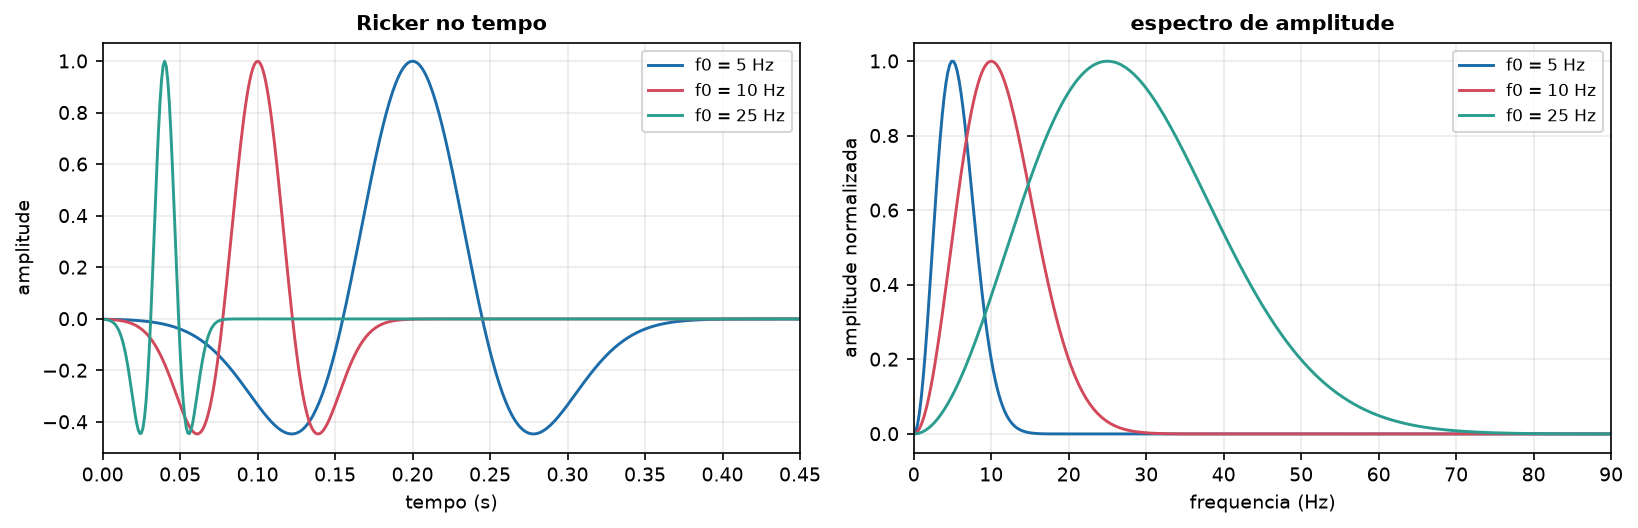
\includegraphics[width=0.96\textwidth]{../saidas/aula01/01_ricker_tempo_frequencia.png}
\caption{A ondaleta de Ricker no tempo e na frequ\^encia, para tr\^es valores
de $f_0$, calculada pelo c\'odigo do curso. Aumentar $f_0$ estreita o pulso
no tempo e alarga o espectro --- a rela\c{c}\~ao rec\'iproca que est\'a por
tr\'as de tudo neste cap\'itulo.}
\end{figure}

\begin{resumo}
\begin{itemize}[leftmargin=*, itemsep=1pt]
\item Um s\'olido carrega ondas P (compress\~ao) e S (cisalhamento); um
fluido, apenas P.
\item A aproxima\c{c}\~ao ac\'ustica \'e \emph{uma} hip\'otese: $\mu=0$, a
rocha tratada como fluido. Dela decorre uma \'unica equa\c{c}\~ao escalar,
para a press\~ao.
\item Ela preserva a cinem\'atica da onda P e descarta ondas S,
convers\~oes, ondas de superf\'icie e atenua\c{c}\~ao.
\item O que a f\'isica n\~ao explica vai para o res\'iduo, e o res\'iduo vira
estrutura falsa no modelo.
\item A fonte tem uma frequ\^encia de pico $f_0$; resolu\c{c}\~ao $\approx
\lambda/2 = c/2f$.
\end{itemize}
\end{resumo}

\begin{exercicio}
\begin{enumerate}[leftmargin=*, itemsep=2pt]
\item Por que a onda S n\~ao existe na \'agua?
\item Um alvo tem 30\,m de espessura, a 2\,km de profundidade, num meio de
2500\,m/s. Qual frequ\^encia \'e necess\'aria para resolv\^e-lo?
\item Um levantamento terrestre foi invertido com FWI ac\'ustica e o modelo
final tem uma camada de baixa velocidade estranha, bem rasa, logo abaixo dos
receptores. Qual \'e a primeira suspeita?
\end{enumerate}
\textbf{Respostas.} (1) Porque a \'agua n\~ao resiste ao cisalhamento
($\mu=0$): n\~ao h\'a for\c{c}a restauradora para o movimento transversal.
(2) $\lambda/2 = 30 \Rightarrow \lambda = 60$\,m $\Rightarrow f = c/\lambda
\approx 42$\,Hz. (3) Onda de superf\'icie (\emph{ground roll}) n\~ao removida:
ela \'e lenta, rasa e intensa, e o modelo ac\'ustico n\~ao tem como
produzi-la a n\~ao ser inventando uma camada lenta.
\end{exercicio}

% =====================================================================
\chapter{Resolver a equa\c{c}\~ao no computador}
\label{cap:numerico}

\begin{ideia}
O computador n\~ao conhece o espa\c{c}o cont\'inuo: ele guarda a press\~ao em
uma grade de pontos e avan\c{c}a em pulinhos de tempo. Duas regras decidem se
o resultado \'e confi\'avel --- uma diz se a simula\c{c}\~ao \emph{roda}, a
outra diz se ela est\'a \emph{certa}.
\end{ideia}

\section{A ideia da grade}

Cobre-se a regi\~ao de interesse com uma grade de pontos espa\c{c}ados de
$\Delta h$, e guarda-se um valor de press\~ao em cada um. O tempo tamb\'em
vira uma sequ\^encia de instantes espa\c{c}ados de $\Delta t$. A regra de
avan\c{c}o \'e simples de descrever:

\begin{center}
\emph{a press\~ao de cada ponto no pr\'oximo instante \'e calculada a partir
da press\~ao dele e dos vizinhos nos dois instantes anteriores.}
\end{center}

\begin{center}
\begin{tikzpicture}[scale=0.85]
\foreach \x in {0,...,8} \foreach \y in {0,...,4}
  \fill[gray!35] (\x,\y) circle (0.055);
\node[circle, draw=vermelhofwi, fill=vermelhofwi!18, line width=1pt,
      inner sep=2.2pt] (c) at (4,2) {};
\foreach \d in {1,2} {
  \fill[cianofwi] (4-\d,2) circle (0.085);
  \fill[cianofwi] (4+\d,2) circle (0.085);
  \fill[cianofwi] (4,2-\d) circle (0.085);
  \fill[cianofwi] (4,2+\d) circle (0.085);
}
\draw[gray!55, <->] (0,-0.55) -- (1,-0.55);
\node[font=\scriptsize, gray!70, below] at (0.5,-0.55) {$\Delta h$};
\node[font=\scriptsize, vermelhofwi, right=4pt] at (4.15,2.45) {ponto atualizado};
\node[font=\scriptsize, cianofwi, right=3pt] at (6.2,2) {vizinhos consultados};
\draw[cianofwi!70, ->, line width=0.6pt] (6.15,2) -- (5.1,2);
\node[font=\scriptsize, gray!75, align=left] at (11.2,3.2)
  {\textbf{est\^encil}: quantos vizinhos\\entram na conta.\\Mais vizinhos =
   mais preciso\\(e mais caro por ponto).};
\end{tikzpicture}
\end{center}

O conjunto de vizinhos consultados chama-se \textbf{est\^encil}, e o seu
tamanho \'e a \textbf{ordem} do esquema. Um est\^encil de 3 pontos por
dire\c{c}\~ao \'e ordem 2; de 5 pontos, ordem 4; de 9 pontos, ordem 8.

\begin{teoria}[Por que ordem alta compensa]
Ordem maior n\~ao serve apenas para ``ser mais preciso''. Serve para ser mais
preciso \textbf{com a mesma grade} --- e, portanto, para permitir uma grade
\emph{mais grossa} com a mesma qualidade.

Isso \'e economia real. Em 2D, dobrar o espa\c{c}amento $\Delta h$ divide o
n\'umero de pontos por 4 \emph{e} permite dobrar o passo de tempo: a
simula\c{c}\~ao fica cerca de \textbf{8 vezes} mais barata. Em 3D, 16 vezes.

Duas ressalvas, para a conta ficar honesta: um est\^encil maior custa mais
opera\c{c}\~oes \emph{por ponto} (ordem 8 usa cerca de 3 vezes mais que ordem
2), e reduz um pouco o passo de tempo m\'aximo (§\ref{sec:cfl1v}). O saldo
continua claramente favor\'avel --- o Volume 2 fecha a conta com todos os
fatores.
\end{teoria}

\begin{matematica}[por que trocar o cont\'inuo pela grade pode dar errado]
Substituir o espa\c{c}o cont\'inuo por uma grade de pontos parece inofensivo,
e n\~ao \'e. Vale entender o tipo de erro que isso cria \emph{antes} das duas
regras.

\textbf{Aproximar uma derivada.} A derivada \'e o limite de
$[f(x+h)-f(x-h)]/2h$ quando $h\to 0$. Numa grade, $h$ n\~ao vai a zero: ele
vale $\Delta h$, e p\'ara ali. Sobra um erro, e o tamanho desse erro depende
de $\Delta h$ e de quantos vizinhos voc\^e consultou.

\textbf{Dois erros diferentes, com consequ\^encias diferentes.} \'E a
distin\c{c}\~ao central deste cap\'itulo:
\begin{itemize}[leftmargin=*, itemsep=1pt]
\item um erro que \textbf{cresce} a cada passo de tempo --- dobra, quadruplica,
e em pouco tempo o programa devolve lixo. \'E a \emph{instabilidade};
\item um erro que \textbf{n\~ao cresce} mas est\'a l\'a, deformando a onda aos
poucos. \'E a \emph{dispers\~ao}.
\end{itemize}
O primeiro voc\^e percebe de imediato, porque tudo explode. O segundo
\textbf{n\~ao d\'a nenhum sinal} --- e \'e por isso que \'e mais perigoso.

\textbf{Uma grandeza sem unidade.} Nas duas regras aparecem n\'umeros como
$C = c\,\Delta t/\Delta h$ (velocidade vezes tempo dividido por dist\^ancia:
as unidades se cancelam) e $G = \lambda/\Delta h$ (dist\^ancia dividida por
dist\^ancia). Grandezas adimensionais como essas valem o mesmo em qualquer
escala do problema --- \'e por isso que d\'a para tabelar um limite \'unico
que serve para todo modelo.
\end{matematica}

\section{Regra 1 --- estabilidade: a condi\c{c}\~ao CFL}
\label{sec:cfl1v}

A primeira regra decide se a simula\c{c}\~ao \emph{sobrevive}. Se o passo de
tempo for grande demais, os valores da grade come\c{c}am a crescer a cada
passo, dobram, quadruplicam, e em poucos milhares de passos o programa
devolve \texttt{NaN} --- ``n\~ao \'e um n\'umero''.

A intui\c{c}\~ao \'e geom\'etrica: em um passo de tempo, a informa\c{c}\~ao
f\'isica viaja a dist\^ancia $c\,\Delta t$. Se essa dist\^ancia ultrapassar o
alcance do est\^encil, a onda estaria ``pulando por cima'' de pontos que o
esquema nunca consultou --- e o resultado n\~ao tem como estar certo. A conta
vira um n\'umero adimensional, o \textbf{n\'umero de Courant}:
\begin{equation}
C = \frac{c_{\max}\,\Delta t}{\Delta h} \;\le\; C_{\lim}.
\label{eq:cfl1}
\end{equation}

Em 2D, os limites s\~ao $C_{\lim} \approx 0{,}71$ (ordem 2), $0{,}61$ (ordem
4) e $0{,}55$ (ordem 8).

Note que esses valores s\~ao \emph{menores} que 1: o argumento geom\'etrico
acima d\'a apenas uma condi\c{c}\~ao \textbf{necess\'aria}, e o limite
verdadeiro --- obtido de uma an\'alise de estabilidade, que o Volume 2 faz ---
\'e mais apertado do que ela.

\begin{atencao}[Duas leituras contraintuitivas]
\textbf{(a) Ordem espacial maior \emph{reduz} o passo de tempo m\'aximo.} O
est\^encil mais largo \'e mais sens\'ivel \`as oscila\c{c}\~oes curtas, e a
condi\c{c}\~ao aperta. Voc\^e ganha em $\Delta h$ e paga em $\Delta t$ ---
mas o saldo continua favor\'avel.

\textbf{(b) Quem manda \'e a velocidade \emph{m\'axima} do modelo.} Uma
\'unica c\'elula r\'apida --- uma camada de sal, um basalto, um erro de
interpola\c{c}\~ao --- derruba o passo de tempo do modelo inteiro.
\end{atencao}

\begin{armadilha}[N\~ao existe ``um pouco inst\'avel'']
A transi\c{c}\~ao \emph{n\~ao} \'e gradual. Medindo com o c\'odigo do curso,
para um esquema com $C_{\lim}=0{,}61$: $C = 0{,}31$ e $C = 0{,}55$ rodam
perfeitamente; $C = 0{,}63$ e $C = 0{,}70$ produzem \texttt{NaN}. Ou est\'a
est\'avel, ou explode.

Use sempre uma margem de 10\% a 20\% abaixo do limite.
\end{armadilha}

\section{Regra 2 --- dispers\~ao: o erro que parece geologia}

A segunda regra decide se a simula\c{c}\~ao est\'a \emph{certa}, e \'e mais
insidiosa, porque quando ela \'e violada \textbf{nada d\'a errado}: a
simula\c{c}\~ao roda at\'e o fim e devolve tra\c{c}os bonitos.

Na equa\c{c}\~ao verdadeira, todas as frequ\^encias viajam com a mesma
velocidade $c$. Na grade, n\~ao: as componentes de comprimento de onda curto
--- as que ``cabem mal'' na grade --- viajam com velocidade ligeiramente
errada. O pulso, que deveria manter a forma, vai se desfazendo e criando uma
\textbf{cauda oscilat\'oria} atr\'as da frente de onda.

\begin{center}
\begin{tikzpicture}[scale=1.0]
\node[font=\small\bfseries, verdefwi] at (2.0,1.5) {grade fina: correto};
\draw[gray!35] (0,0) -- (4.6,0);
\draw[verdefwi, line width=1.1pt, domain=0:4.6, samples=200, smooth]
  plot (\x, {0.9*(1-2*(pi*1.4*(\x-2.3))^2)*exp(-(pi*1.4*(\x-2.3))^2)});
\begin{scope}[xshift=6.4cm]
\node[font=\small\bfseries, vermelhofwi] at (2.0,1.5) {grade grossa: disperso};
\draw[gray!35] (0,0) -- (4.6,0);
\draw[vermelhofwi, line width=1.1pt, domain=0:4.6, samples=300, smooth]
  plot (\x, {0.9*(1-2*(pi*1.4*(\x-2.3))^2)*exp(-(pi*1.4*(\x-2.3))^2)
            + 0.30*exp(-0.55*max(0,\x-2.3))*sin(deg(9*(\x-2.3)))*(\x>2.3)});
\draw[gray!70, ->, line width=0.6pt] (4.3,1.05) -- (3.5,0.35);
\node[font=\scriptsize, gray!75, right] at (3.9,1.2) {cauda falsa};
\end{scope}
\end{tikzpicture}
\end{center}

\begin{armadilha}[Por que isso \'e perigoso, e n\~ao apenas feio]
A cauda dispersiva \textbf{parece sinal}: reverbera\c{c}\~ao, camada fina,
\emph{ringing} da fonte. Quem n\~ao conhece o efeito interpreta artefato
num\'erico como geologia. E, pior, a FWI tenta explic\'a-lo com estrutura no
modelo.

\textbf{O teste decisivo, e \'e barato:} simule num meio \emph{homog\^eneo}.
N\~ao h\'a nada para refletir. Qualquer oscila\c{c}\~ao depois do primeiro
pulso \'e erro num\'erico, ponto final.
\end{armadilha}

O controle \'e o n\'umero de \textbf{pontos por comprimento de onda}:
\begin{equation}
G = \frac{\lambda_{\min}}{\Delta h},
\qquad
G \gtrsim
\begin{cases}
15\text{--}20 & \text{ordem 2}\\
8\text{--}10  & \text{ordem 4}\\
4\text{--}5   & \text{ordem 8}
\end{cases}
\label{eq:G}
\end{equation}

Ou seja: a grade tem de ser fina o bastante para que a \emph{menor} onda
presente na simula\c{c}\~ao seja descrita por um punhado de pontos.

\begin{figure}[htbp]
\centering
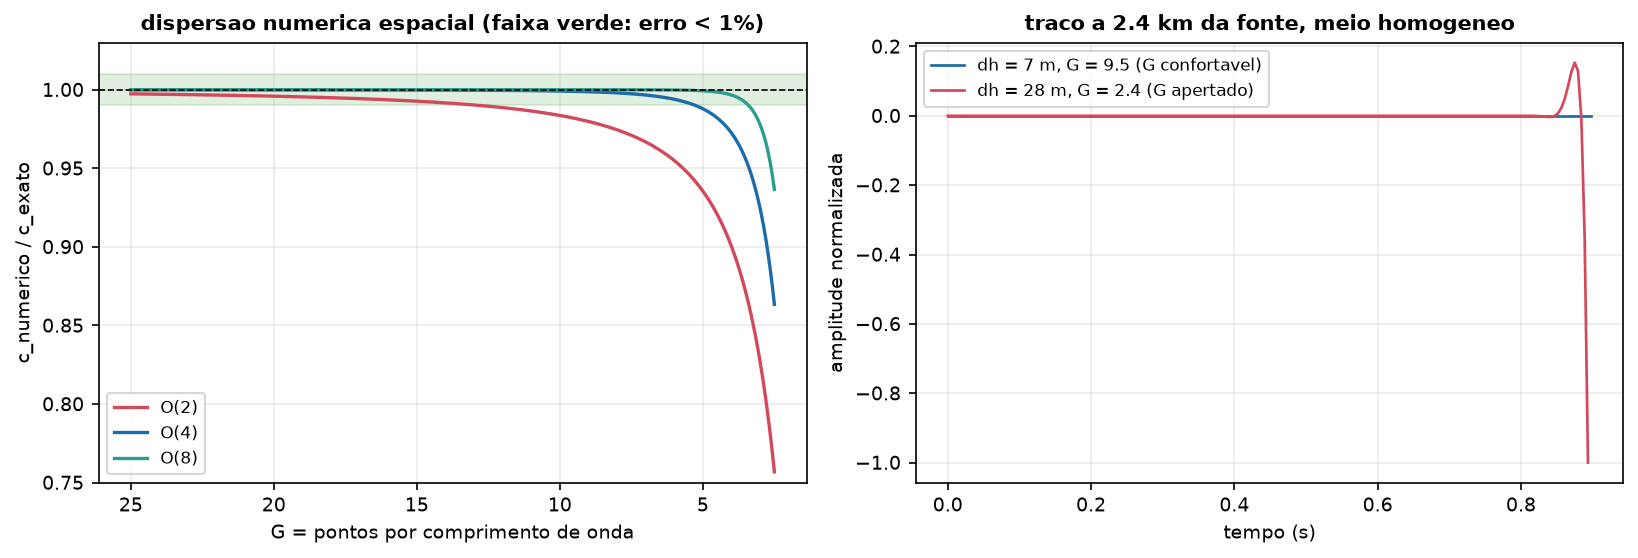
\includegraphics[width=0.96\textwidth]{../saidas/aula02/01_dispersao_numerica.png}
\caption{\`A esquerda: o quanto a velocidade da grade se afasta da velocidade
verdadeira, em fun\c{c}\~ao de quantos pontos descrevem um comprimento de
onda, para tr\^es ordens. \`A direita: um tra\c{c}o real a 2{,}3\,km da fonte
em meio homog\^eneo, com grade boa ($G=9{,}5$) e ruim ($G=2{,}4$). A cauda do
tra\c{c}o vermelho n\~ao existe na f\'isica.}
\end{figure}

\begin{atencao}[Um detalhe que muitos textos omitem]
A curva da figura acima descreve apenas o erro do est\^encil \emph{espacial}.
A discretiza\c{c}\~ao do \emph{tempo} acrescenta um erro pr\'oprio, de sinal
oposto --- e perto do limite CFL, especialmente em ordem 8, \'e o erro
temporal que domina. Na pr\'atica: n\~ao confie na curva espacial como se
fosse conservadora; use margem.
\end{atencao}

\ponte{N\'ivel 2, §3.3}{a rela\c{c}\~ao de dispers\~ao do esquema completo
(espa\c{c}o \emph{e} tempo), com os n\'umeros que mostram quando um erro
cancela o outro.}

\section{A receita de dimensionamento}

Juntando as duas regras, sai um procedimento mec\^anico. \'E o que se faz
antes de \emph{qualquer} simula\c{c}\~ao:

\begin{enumerate}[leftmargin=*]
\item Estime a maior frequ\^encia com energia relevante:
$f_{\max} \approx 2{,}5\,f_0$ para uma Ricker.
\item Calcule o menor comprimento de onda presente:
$\lambda_{\min} = c_{\min}/f_{\max}$ --- com a \emph{menor} velocidade do
modelo.
\item Escolha $\Delta h = \lambda_{\min}/G$, com $G$ da tabela
\eqref{eq:G}.
\item Escolha $\Delta t = 0{,}9\,C_{\lim}\,\Delta h / c_{\max}$ --- com a
\emph{maior} velocidade do modelo.
\end{enumerate}

\begin{atencao}[O conflito embutido, que nenhuma escolha resolve]
A grade \'e ditada pela velocidade \textbf{m\'inima} e o passo de tempo pela
velocidade \textbf{m\'axima}. Um modelo com grande contraste --- \'agua a
1500\,m/s e sal a 4500\,m/s --- \'e caro dos dois lados ao mesmo tempo:
precisa de grade fina por causa da \'agua e de passo curto por causa do sal.

Essa tens\~ao \'e a raz\~ao pr\'atica de existirem malhas de espa\c{c}amento
vari\'avel e esquemas mais sofisticados.
\end{atencao}

\begin{resumo}
\begin{itemize}[leftmargin=*, itemsep=1pt]
\item A simula\c{c}\~ao guarda a press\~ao numa grade e avan\c{c}a em passos
de tempo, consultando vizinhos (o est\^encil).
\item \textbf{Estabilidade} (CFL): $c_{\max}\Delta t/\Delta h \le C_{\lim}$.
Violar produz \texttt{NaN}, sem meio-termo.
\item \textbf{Dispers\~ao}: pontos por comprimento de onda insuficientes
criam uma cauda oscilat\'oria que \emph{parece} geologia. Violar n\~ao produz
erro nenhum --- s\'o um resultado errado.
\item Grade ditada por $c_{\min}$, passo de tempo por $c_{\max}$: modelos de
alto contraste s\~ao caros duas vezes.
\end{itemize}
\end{resumo}

\begin{exercicio}
\begin{enumerate}[leftmargin=*, itemsep=2pt]
\item Modelo com $c$ entre 1500 e 3500\,m/s, fonte de $f_0 = 12$\,Hz, esquema
de ordem 4. Qual $\Delta h$ e qual $\Delta t$?
\item A sua simula\c{c}\~ao rodou e o tra\c{c}o tem uma reverbera\c{c}\~ao
longa. Como saber em cinco minutos se \'e f\'isica ou num\'erica?
\item Voc\^e reduziu $\Delta h$ pela metade para ter mais precis\~ao. Quanto
mais cara ficou a simula\c{c}\~ao em 2D?
\end{enumerate}
\textbf{Respostas.} (1) $f_{\max} = 30$\,Hz; $\lambda_{\min} = 1500/30 =
50$\,m; com $G=8$, $\Delta h = 6{,}25$\,m; $\Delta t = 0{,}9 \times 0{,}61
\times 6{,}25/3500 \approx 0{,}98$\,ms. (2) Rode a mesma fonte num meio
homog\^eneo de velocidade t\'ipica: se a cauda continua l\'a, \'e num\'erica.
(3) Quatro vezes mais pontos e o dobro de passos de tempo (pela CFL): cerca de
8 vezes.
\end{exercicio}

% =====================================================================
\chapter{Bordas, superf\'icie livre e aquisi\c{c}\~ao}
\label{cap:bordas}

\begin{ideia}
A Terra \'e praticamente infinita e o computador tem um peda\c{c}o finito. As
paredes desse peda\c{c}o viram espelhos, e os ecos falsos que elas produzem
entram no res\'iduo como se fossem geologia. Este cap\'itulo trata de apagar
as paredes --- e de onde colocar fontes e receptores.
\end{ideia}

\section{As bordas n\~ao s\~ao detalhe}

Cortar o dom\'inio de simula\c{c}\~ao \'e inevit\'avel. Mas, na borda, a onda
encontra uma descontinuidade abrupta e faz o que qualquer onda faz: reflete.
O resultado \'e um eco que a Terra real nunca produziu.

Em modelagem pura, isso \'e apenas feio. \textbf{Em FWI \'e pior}: o res\'iduo
passa a conter eventos que nenhum modelo pode explicar, e o algoritmo tenta
explic\'a-los mexendo na velocidade. Voc\^e fabrica estrutura falsa --- de
novo o mesmo princ\'ipio do Cap\'itulo~\ref{cap:fisica}.

\begin{center}
\begin{tikzpicture}[scale=0.95]
% dominio com moldura
\fill[vermelhofwi!7] (0,0) rectangle (6.2,4.0);
\fill[white] (0.9,0.9) rectangle (5.3,3.4);
\draw[gray!60] (0,0) rectangle (6.2,4.0);
\draw[vermelhofwi!60, dashed] (0.9,0.9) rectangle (5.3,3.4);
\node[font=\scriptsize, vermelhofwi!80] at (3.1,0.45) {moldura absorvente};
\node[font=\scriptsize, gray!75] at (3.1,3.75) {(dom\'inio f\'isico no centro)};
\fill[vermelhofwi] (3.1,3.0) circle (0.08);
\foreach \r in {0.5,0.95,1.4} \draw[cianofwi!70] (3.1,3.0) circle (\r);
\draw[verdefwi, line width=0.9pt, ->] (3.1,3.0) -- (1.35,1.5);
\node[font=\scriptsize, verdefwi] at (1.9,2.05) {absorvida};
% sem moldura
\begin{scope}[xshift=7.6cm]
\draw[gray!60] (0,0) rectangle (6.2,4.0);
\fill[vermelhofwi] (3.1,3.0) circle (0.08);
\foreach \r in {0.5,0.95,1.4} \draw[cianofwi!70] (3.1,3.0) circle (\r);
\draw[vermelhofwi, line width=0.9pt, ->] (3.1,3.0) -- (0.05,0.4);
\draw[vermelhofwi, line width=0.9pt, ->] (0.05,0.4) -- (2.6,0.4);
\node[font=\scriptsize, vermelhofwi] at (3.6,0.62) {eco falso};
\node[font=\scriptsize, gray!75] at (3.1,3.75) {(sem moldura: espelho)};
\end{scope}
\end{tikzpicture}
\end{center}

A solu\c{c}\~ao \'e cercar o dom\'inio f\'isico com uma \textbf{moldura} cuja
\'unica fun\c{c}\~ao \'e engolir a onda que entra nela. As duas fam\'ilias
mais usadas:

\begin{center}
\begin{tabular}{@{}lp{5.0cm}ll@{}}
\toprule
\textbf{T\'ecnica} & \textbf{Ideia} & \textbf{Custo} & \textbf{Qualidade} \\
\midrule
Truncar & nada & zero & inaceit\'avel \\
\emph{Sponge} (Cerjan) & multiplicar o campo por um fator $<1$ dentro da
moldura, cada vez mais forte & baixo & razo\'avel \\
CPML & reescrever a equa\c{c}\~ao dentro da moldura para que a onda
decaia sem refletir na entrada & m\'edio & excelente \\
\bottomrule
\end{tabular}
\end{center}

Medindo a reflex\~ao residual com o c\'odigo do curso --- comparando cada
caso com uma simula\c{c}\~ao em dom\'inio muito maior, onde nada reflete
dentro da janela de tempo --- a CPML com 10 pontos de moldura j\'a supera com
folga o \emph{sponge} com 45 pontos. \'E por isso que c\'odigos de
produ\c{c}\~ao usam CPML.

\begin{pratica}[A regra de dimensionamento da moldura]
A moldura precisa ter pelo menos \textbf{meio comprimento de onda da menor
frequ\^encia usada}. E como a FWI (Cap.~\ref{cap:misfit}) come\c{c}a de
prop\'osito pelas frequ\^encias baixas, dimensione por $f_{\min}$ --- nunca
por $f_0$. Moldura curta demais \'e um erro que s\'o aparece na primeira banda
da invers\~ao, quando j\'a \'e tarde.
\end{pratica}

\section{A superf\'icie livre: uma escolha f\'isica, n\~ao num\'erica}

No topo do modelo a decis\~ao \'e diferente, porque ali existe uma interface
\emph{de verdade}: a superf\'icie da Terra, ou do mar.

\begin{itemize}[leftmargin=*]
\item \textbf{Superf\'icie livre} ($p=0$ no topo): representa o contato com o
ar. A onda reflete com polaridade invertida. Isso produz as
\textbf{m\'ultiplas} de superf\'icie e o \emph{ghost} --- que s\~ao eventos
\emph{reais}, presentes no dado gravado.
\item \textbf{Moldura absorvente no topo}: representa um meio que continua
para cima indefinidamente. N\~ao \'e f\'isico, mas elimina as m\'ultiplas do
sint\'etico.
\end{itemize}

\begin{armadilha}[O erro de consist\^encia]
Se o dado observado cont\'em m\'ultiplas e o sint\'etico n\~ao, a
\emph{diferen\c{c}a inteira} vai para o res\'iduo, e a FWI vai tentar
reproduzir m\'ultiplas mexendo na velocidade.

H\'a duas sa\'idas leg\'itimas: modelar a superf\'icie livre, ou remover as
m\'ultiplas do dado antes de inverter. Ignorar a quest\~ao n\~ao \'e uma
delas.
\end{armadilha}

\section{Aquisi\c{c}\~ao: onde p\^or fontes e receptores}
\label{sec:aquisicao}

\begin{figure}[htbp]
\centering
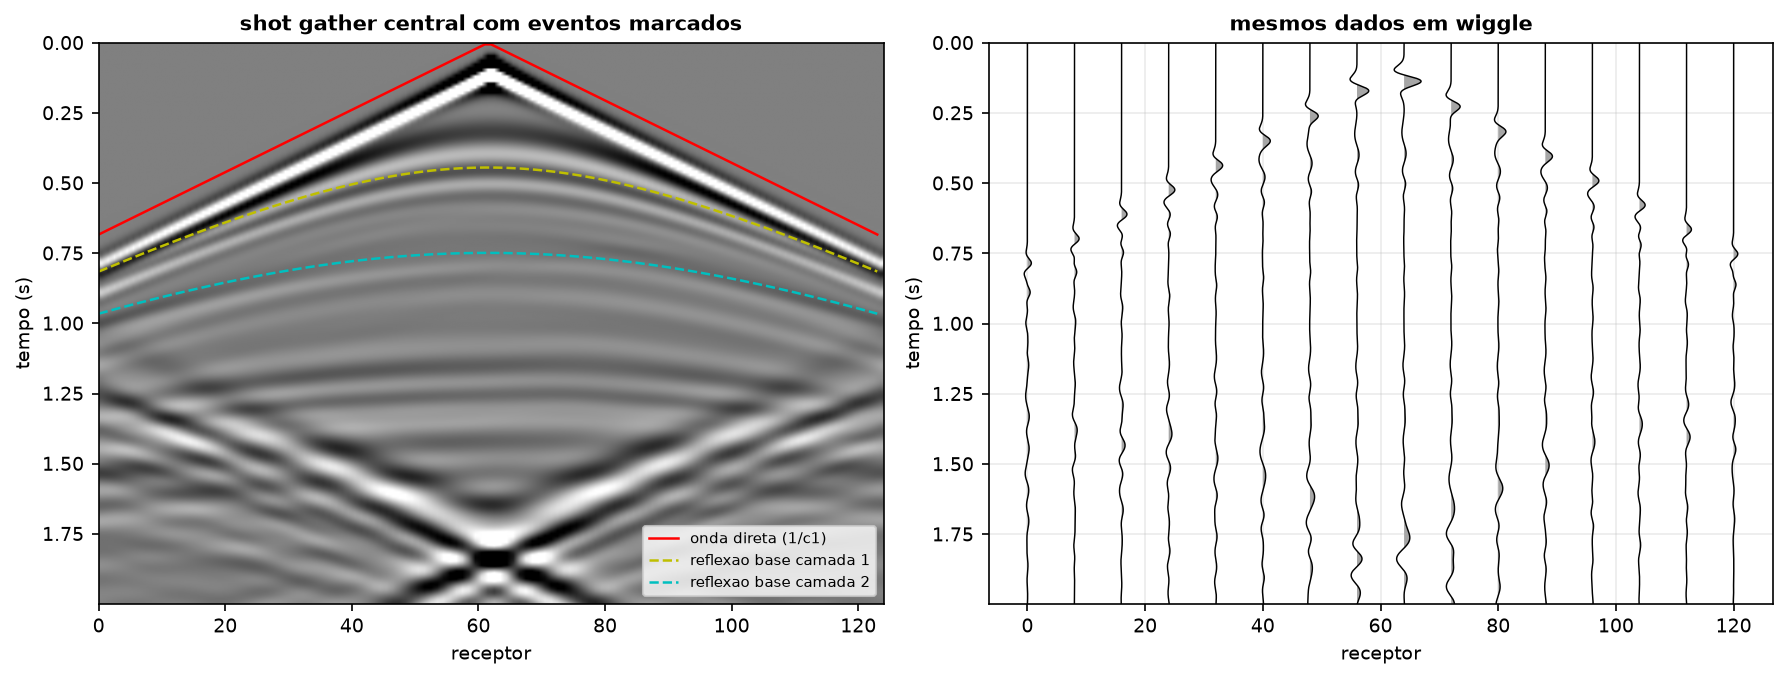
\includegraphics[width=0.95\textwidth]{../saidas/aula04/02_anatomia_shot_gather.png}
\caption{Anatomia de um registro de um \'unico disparo (\emph{shot gather}),
com as curvas te\'oricas sobrepostas. Cada coluna \'e um receptor; o tempo
cresce para baixo.}
\end{figure}

Um \emph{shot gather} \'e o registro de um \'unico disparo em todos os
receptores. Nele, cada fam\'ilia de ondas tem uma assinatura geom\'etrica
reconhec\'ivel:

\begin{itemize}[leftmargin=*]
\item \textbf{onda direta} --- uma reta saindo da origem: a onda que vai da
fonte ao receptor sem descer. N\~ao carrega informa\c{c}\~ao de profundidade;
\item \textbf{refra\c{c}\~oes} --- retas produzidas por ondas que mergulharam
numa camada mais r\'apida e voltaram. S\~ao duas dist\^ancias diferentes, e
confundi-las \'e comum: elas s\'o \emph{come\c{c}am a existir} a partir da
dist\^ancia cr\'itica, e s\'o mais longe ainda --- na dist\^ancia de
cruzamento --- passam a chegar \emph{antes} da direta. S\~ao a fonte mais rica
de informa\c{c}\~ao sobre a velocidade de grande escala;
\item \textbf{reflex\~oes} --- hip\'erboles: a curvatura revela a velocidade
m\'edia at\'e o refletor;
\item \textbf{difra\c{c}\~oes} --- hip\'erboles de \'apice deslocado,
produzidas por pontos isolados: falhas, quinas, corpos pequenos.
\end{itemize}

\begin{teoria}[A rela\c{c}\~ao mais \'util da aquisi\c{c}\~ao]
\[
\text{profundidade confi\'avel} \;\approx\;
\frac{\text{afastamento m\'aximo}}{3}\ \text{a}\
\frac{\text{afastamento m\'aximo}}{2}.
\]

A raz\~ao \'e geom\'etrica. Para separar ``mais lento e mais raso'' de ``mais
r\'apido e mais fundo'' \'e preciso iluminar cada ponto com \^angulos
\emph{variados}, e \^angulos variados exigem raios vindo de longe.
Afastamento curto s\'o produz incid\^encia quase normal, que \'e amb\'igua.

\textbf{Consequ\^encia pr\'atica:} para enxergar mais fundo, aumente o
\emph{afastamento}. Receptores mais densos combatem \emph{aliasing}; mais
disparos melhoram a raz\~ao sinal/ru\'ido; frequ\^encia maior melhora a
resolu\c{c}\~ao. Nenhum dos tr\^es ilumina mais fundo.
\end{teoria}

\begin{atencao}[Por que a FWI nunca usa dado empilhado]
A FWI trabalha \emph{sempre} com disparo por disparo, e a raz\~ao \'e
conceitual: o simulador $F$ modela um disparo por vez, ent\~ao o res\'iduo
tem de ser calculado nessa mesma organiza\c{c}\~ao.

Al\'em disso, o empilhamento descarta justamente a depend\^encia com o
afastamento --- que \'e a informa\c{c}\~ao que separa velocidade de
profundidade.
\end{atencao}

\subsection*{Dois cuidados de amostragem}

\textbf{Espa\c{c}amento entre receptores.} Se os receptores estiverem muito
distantes entre si, eventos inclinados deixam de ser cont\'inuos de um
tra\c{c}o para o outro: \'e o \emph{aliasing} espacial. Em FWI isso \'e
especialmente perverso, porque a invers\~ao tenta explicar o padr\~ao
serrilhado com estrutura no modelo.

\textbf{Ru\'ido.} A FWI tolera bem ru\'ido \emph{aleat\'orio} --- ele n\~ao
soma coerentemente no gradiente quando se empilham muitos disparos. O que ela
n\~ao tolera \'e ru\'ido \textbf{coerente} e erro sistem\'atico de modelagem:
esses somam em fase e viram estrutura.

\begin{resumo}
\begin{itemize}[leftmargin=*, itemsep=1pt]
\item As bordas do dom\'inio refletem; a moldura absorvente existe para
apagar esse eco, e deve ser dimensionada pela \emph{menor} frequ\^encia.
\item A superf\'icie do topo \'e uma escolha f\'isica: superf\'icie livre
(com m\'ultiplas) ou absorvente (sem). O sint\'etico e o dado observado
precisam concordar.
\item A FWI trabalha disparo a disparo, nunca com dado empilhado.
\item Profundidade de investiga\c{c}\~ao $\approx$ um ter\c{c}o a metade do
maior afastamento. Densidade de receptores e frequ\^encia n\~ao mudam isso.
\item Ru\'ido aleat\'orio \'e tolerado; ru\'ido coerente e erro de modelagem
viram geologia falsa.
\end{itemize}
\end{resumo}

% =====================================================================
\part*{\centering\color{azulfwi} Parte II --- A invers\~ao: o problema inverso}
\addcontentsline{toc}{part}{Parte II --- A invers\~ao: o problema inverso}

\chapter{A fun\c{c}\~ao objetivo e o \emph{cycle skipping}}
\label{cap:misfit}

\begin{ideia}
Medir a discord\^ancia entre sint\'etico e observado amostra a amostra \'e a
escolha mais natural do mundo --- e \'e ela que cria o principal modo de
falha da FWI. Se o sint\'etico estiver atrasado por mais de \emph{meio
per\'iodo}, a corre\c{c}\~ao aponta para o lado errado.
\end{ideia}

\section{A paisagem que o algoritmo percorre}

Pense em $J(\mvec)$ como uma paisagem montanhosa: cada modelo poss\'ivel \'e
um ponto no ch\~ao, e a altura \'e o qu\~ao mal aquele modelo explica os
dados. Procurar o modelo certo \'e procurar o fundo do vale --- \emph{no
escuro}, sabendo apenas a inclina\c{c}\~ao sob os seus p\'es.

Descer sempre pela inclina\c{c}\~ao funciona se a paisagem for uma tigela.
N\~ao funciona se houver v\'arios vales: voc\^e chega ao fundo do vale mais
pr\'oximo, n\~ao ao mais baixo.

\begin{figure}[htbp]
\centering
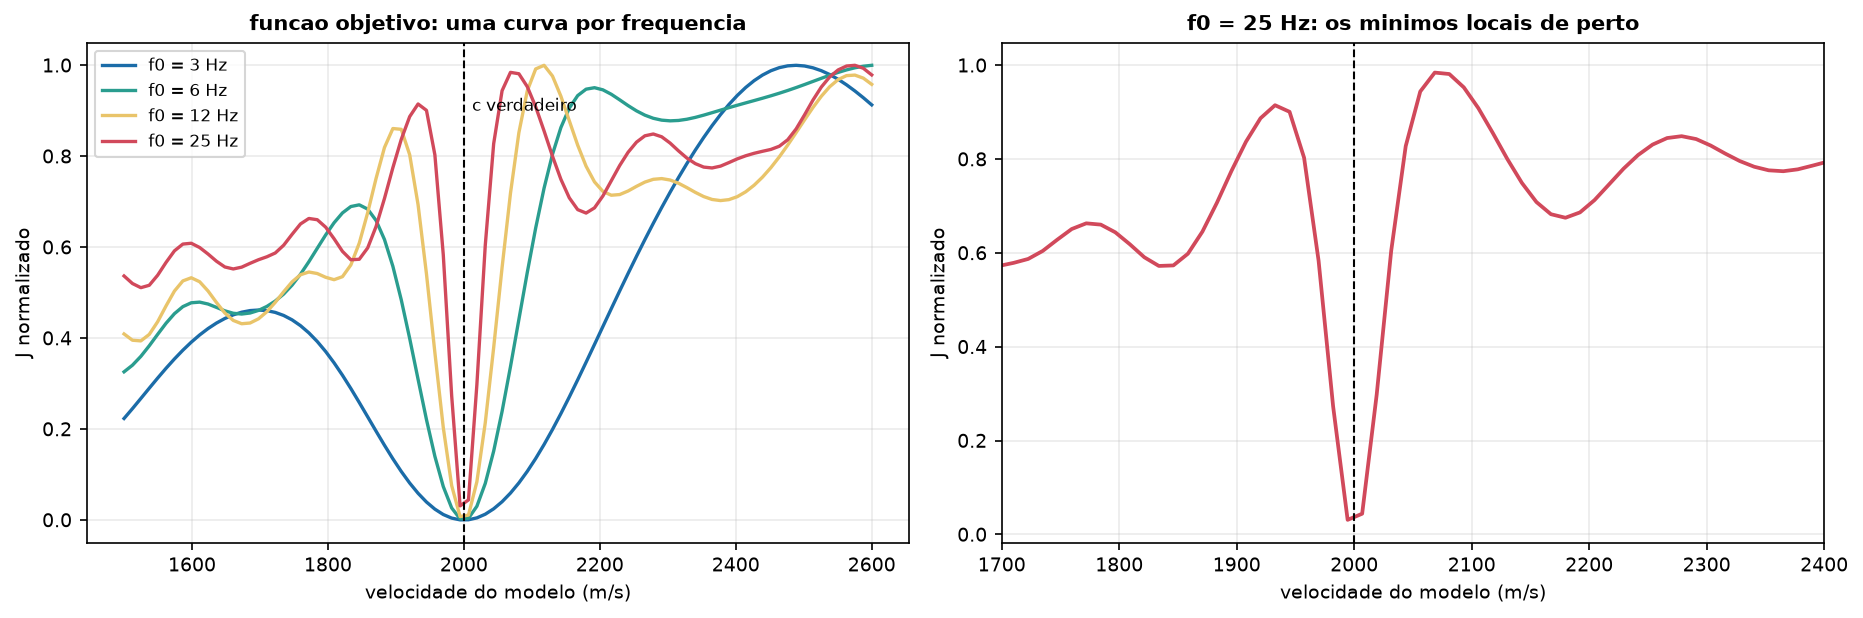
\includegraphics[width=0.95\textwidth]{../saidas/aula07/01_funcao_objetivo.png}
\caption{A paisagem, desenhada de verdade. Num meio homog\^eneo h\'a um
\'unico par\^ametro --- a velocidade --- e \'e poss\'ivel varr\^e-lo e
desenhar $J$ inteiro, coisa imposs\'ivel com um milh\~ao de par\^ametros. Em
\textbf{baixa} frequ\^encia: um vale largo e \'unico. Em \textbf{alta}
frequ\^encia: um vale estreito cercado de m\'inimos locais. A velocidade
verdadeira \'e 2000\,m/s nos quatro pain\'eis.}
\end{figure}

Essa figura cont\'em a ideia pr\'atica mais importante de toda a
cole\c{c}\~ao. \textbf{A forma da paisagem depende da frequ\^encia}, e a
frequ\^encia \'e escolha sua.

\begin{matematica}[per\'iodo, fase e defasagem]
O argumento a seguir \'e todo sobre \emph{alinhamento no tempo}. Tr\^es
palavras bastam.

\textbf{Per\'iodo.} Uma onda de frequ\^encia $f$ repete o seu padr\~ao a cada
$T = 1/f$ segundos. A 10\,Hz, $T = 0{,}1$\,s; a 40\,Hz, $T = 0{,}025$\,s.
Quanto maior a frequ\^encia, mais curto o per\'iodo --- e \'e por isso que
frequ\^encia alta \'e menos tolerante a erro.

\textbf{Defasagem.} \'E o deslocamento no tempo entre dois sinais parecidos.
Se o sint\'etico chega $\delta t$ depois do observado, $\delta t$ \'e a
defasagem.

\textbf{Por que ``meio per\'iodo'' \'e a fronteira.} Uma onda \'e
\emph{repetitiva}: ela tem v\'arios lobos parecidos entre si. Quando dois
sinais repetitivos s\~ao comparados, o que importa n\~ao \'e s\'o ``o
quanto est\~ao separados'', mas \emph{qual lobo est\'a mais perto de qual}.
Enquanto a separa\c{c}\~ao for menor que meio per\'iodo, o lobo mais pr\'oximo
ainda \'e o correspondente. Passando disso, o vizinho fica mais perto --- e o
algoritmo, que s\'o sabe aproximar o que est\'a perto, alinha com o vizinho
errado.

\'E o mesmo fen\^omeno de quem afina um instrumento por compara\c{c}\~ao e
acaba afinando uma oitava acima: a compara\c{c}\~ao local est\'a certa, a
identifica\c{c}\~ao do par \'e que estava errada.
\end{matematica}

\section{A causa: meio per\'iodo}

Por que a alta frequ\^encia cria m\'inimos locais? A explica\c{c}\~ao \'e
puramente de \textbf{fase}, e cabe em um desenho.

Suponha que o modelo esteja um pouco errado, de modo que o pulso sint\'etico
chegue deslocado de $\delta t$ em rela\c{c}\~ao ao observado. O algoritmo vai
tentar alinhar os dois. A pergunta \'e: \emph{alinhar com qual ciclo?}

\begin{center}
\begin{tikzpicture}
\begin{axis}[width=7.4cm, height=4.4cm, title={\small deslocamento
  $<$ meio per\'iodo: \textcolor{verdefwi}{corrige certo}},
  xmin=0, xmax=0.5, ymin=-0.8, ymax=1.2, axis lines=left, grid=both,
  grid style={gray!15}, xlabel={$t$}, ylabel={amplitude},
  label style={font=\scriptsize}, tick label style={font=\scriptsize},
  title style={font=\small}, legend style={font=\scriptsize, draw=gray!40,
  at={(0.98,0.98)}, anchor=north east}, samples=300, domain=0:0.5]
\addplot[azulfwi, line width=1pt]
  {(1-2*(pi*10*(x-0.22))^2)*exp(-(pi*10*(x-0.22))^2)};
\addlegendentry{observado}
\addplot[vermelhofwi, line width=1pt, dashed]
  {(1-2*(pi*10*(x-0.25))^2)*exp(-(pi*10*(x-0.25))^2)};
\addlegendentry{sint\'etico}
\draw[verdefwi, line width=1pt, {Stealth[length=2mm]}-{Stealth[length=2mm]}]
  (axis cs:0.22,-0.65) -- (axis cs:0.25,-0.65);
\end{axis}
\end{tikzpicture}
\hfill
\begin{tikzpicture}
\begin{axis}[width=7.4cm, height=4.4cm, title={\small deslocamento
  $>$ meio per\'iodo: \textcolor{vermelhofwi}{corrige errado}},
  xmin=0, xmax=0.5, ymin=-0.8, ymax=1.2, axis lines=left, grid=both,
  grid style={gray!15}, xlabel={$t$},
  label style={font=\scriptsize}, tick label style={font=\scriptsize},
  title style={font=\small}, legend style={font=\scriptsize, draw=gray!40,
  at={(0.98,0.98)}, anchor=north east}, samples=300, domain=0:0.5]
\addplot[azulfwi, line width=1pt]
  {(1-2*(pi*10*(x-0.18))^2)*exp(-(pi*10*(x-0.18))^2)};
\addlegendentry{observado}
\addplot[vermelhofwi, line width=1pt, dashed]
  {(1-2*(pi*10*(x-0.25))^2)*exp(-(pi*10*(x-0.25))^2)};
\addlegendentry{sint\'etico}
\draw[vermelhofwi, line width=1pt, -{Stealth[length=2mm]}]
  (axis cs:0.25,-0.65) -- (axis cs:0.33,-0.65);
\node[font=\scriptsize, vermelhofwi] at (axis cs:0.40,-0.45)
  {vai para c\'a};
\end{axis}
\end{tikzpicture}
\end{center}

\`A esquerda, o lobo principal do sint\'etico ainda se sobrep\~oe ao lobo
principal do observado: puxar o sint\'etico para a esquerda diminui o
res\'iduo, e o algoritmo faz a coisa certa. \`A direita, o sint\'etico
atrasou tanto que o lobo dele encontrou o lobo \emph{seguinte} do observado:
agora \'e empurr\'a-lo mais para a direita que diminui o res\'iduo. O
algoritmo desce para o vale errado, com total convic\c{c}\~ao.

\begin{teoria}[O crit\'erio de meio ciclo]
Para um pulso de frequ\^encia dominante $f$ (per\'iodo $T = 1/f$), a
invers\~ao s\'o corrige na dire\c{c}\~ao certa se
\begin{equation}
\boxed{\ \abs{\delta t} < \frac{T}{2} = \frac{1}{2f}\ }
\label{eq:meiociclo1}
\end{equation}

Esta \'e, sem exagero, a desigualdade mais importante da pr\'atica de FWI.
Tudo o que se faz de estrat\'egia --- multiescala, modelo inicial,
funcionais alternativos --- existe para manter $\abs{\delta t}$ desse lado da
conta.
\end{teoria}

\begin{atencao}[Meio per\'iodo \'e uma regra pr\'atica, e sabe-se o quanto]
O ``meio per\'iodo'' vale exatamente para um pulso harm\^onico. Para uma
ondaleta real ele \'e uma aproxima\c{c}\~ao --- boa, mas aproxima\c{c}\~ao.

Calculando $J$ para uma Ricker deslocada de $\delta t$, a divisa entre
``corrige certo'' e ``corrige errado'' fica em $\delta t \approx 0{,}43\,T$
(um pouco \emph{antes} de meio per\'iodo), e h\'a um m\'inimo local esp\'urio
em $\delta t \approx 0{,}9\,T$ --- que \'e, literalmente, o vale errado em
que a invers\~ao cai.

Ou seja: a regra de meio per\'iodo \'e ligeiramente \textbf{otimista}. Use-a
com margem.
\end{atencao}

\section{Traduzindo para o erro de velocidade}

O crit\'erio fica muito mais \'util quando escrito em termos daquilo que
voc\^e controla: o erro do modelo inicial. Para um percurso de comprimento
$L$, o erro de tempo acumulado \'e proporcional ao erro de vagarosidade, e o
crit\'erio \eqref{eq:meiociclo1} vira uma toler\^ancia expl\'icita:
\begin{equation}
\abs{\delta c} < \frac{c^{2}}{2 f L}.
\label{eq:tolerancia1}
\end{equation}

Com $c = 2000$\,m/s e um percurso de $L = 1500$\,m:

\begin{center}
\begin{tabular}{@{}rrrl@{}}
\toprule
$f$ (Hz) & $T/2$ (ms) & erro m\'aximo de $c$ & \\
\midrule
2  & 250{,}0 & 667\,m/s & $33{,}3\%$ --- muito tolerante \\
5  & 100{,}0 & 267\,m/s & $13{,}3\%$ \\
10 & 50{,}0  & 133\,m/s & $6{,}7\%$ \\
20 & 25{,}0  & 67\,m/s  & $3{,}3\%$ \\
40 & 12{,}5  & 33\,m/s  & $1{,}7\%$ --- exigiria j\'a saber a resposta \\
\bottomrule
\end{tabular}
\end{center}

A leitura \'e direta e um pouco brutal: \textbf{a 40\,Hz voc\^e precisaria
come\c{c}ar j\'a sabendo a velocidade com menos de 2\% de erro}. A 2\,Hz,
pode errar um ter\c{c}o.

\begin{pratica}[Use isto \emph{antes} de rodar]
Estime a frequ\^encia mais alta com que voc\^e pode \emph{come\c{c}ar}, dada
a incerteza do seu modelo inicial. Se a tomografia pr\'evia tem 5\% de erro e
o percurso t\'ipico \'e de 2\,km, com $c\approx 2000$\,m/s:
\[
\delta c = 100\ \text{m/s} \;\Longrightarrow\;
f_{\max} = \frac{c^2}{2\,\delta c\,L}
 = \frac{2000^2}{2\cdot 100\cdot 2000} = 10\ \text{Hz}.
\]
Come\c{c}ar acima disso \'e desperdi\c{c}ar tempo de m\'aquina para obter um
resultado errado com apar\^encia de certo.
\end{pratica}

\section{A consequ\^encia: a estrat\'egia multiescala}

De \eqref{eq:meiociclo1} decorre, sem nenhuma hip\'otese adicional, a receita
que organiza toda FWI de produ\c{c}\~ao:

\begin{center}
\begin{tikzpicture}[scale=1.0]
\foreach \i/\f/\lbl in {0/3/{3\,Hz}, 1/6/{6\,Hz}, 2/12/{12\,Hz}, 3/25/{25\,Hz}} {
  \pgfmathsetmacro{\xx}{3.2*\i}
  \pgfmathsetmacro{\w}{1.15*3/\f}
  \draw[gray!45] (\xx,0) -- (\xx+2.7,0);
  \draw[azulfwi, line width=1pt, domain=0:2.7, samples=80, smooth]
    plot (\xx+\x, {1.3*(1 - exp(-((\x-1.35)/\w)^2))});
  \fill[verdefwi] (\xx+1.35,0.02) circle (0.07);
  \draw[verdefwi, line width=0.8pt, |-|]
    (\xx+1.35-\w,-0.28) -- (\xx+1.35+\w,-0.28);
  \node[font=\scriptsize, gray!80] at (\xx+1.35,-0.62) {\lbl};
  \ifnum\i<3
    \draw[-{Stealth[length=2.4mm]}, roxofwi, line width=0.9pt]
      (\xx+1.35,1.75) .. controls (\xx+2.2,2.15) and (\xx+2.6,2.15) ..
      (\xx+3.2+1.35-0.1,1.75);
  \fi
}
\node[font=\scriptsize, roxofwi] at (4.8,2.45)
  {o resultado de uma banda \'e o ponto de partida da seguinte};
\node[font=\scriptsize, verdefwi, anchor=west] at (-0.4,-0.95)
  {largura do vale de atra\c{c}\~ao $\propto 1/f$};
\end{tikzpicture}
\end{center}

\begin{enumerate}[leftmargin=*]
\item Filtre o dado observado para manter s\'o as frequ\^encias mais baixas.
Nessa banda, a paisagem \'e quase uma tigela: quase qualquer modelo inicial
converge.
\item Inverta at\'e convergir. O resultado n\~ao tem resolu\c{c}\~ao, mas tem
as escalas grandes certas.
\item Suba um degrau de frequ\^encia, usando esse resultado como modelo
inicial. Agora o vale \'e mais estreito --- mas voc\^e j\'a est\'a dentro
dele.
\item Repita at\'e a frequ\^encia m\'axima \'util.
\end{enumerate}

\begin{atencao}[Multiescala n\~ao \'e truque num\'erico]
\'E consequ\^encia direta de \eqref{eq:meiociclo1}. E tem um limite honesto:
a estrat\'egia s\'o resgata o que a banda \textbf{mais baixa} j\'a alcan\c{c}a.
Se o modelo inicial estiver fora do vale de atra\c{c}\~ao \emph{da menor
frequ\^encia dispon\'ivel}, nenhuma ordem de bandas salva --- o
Cap\'itulo~\ref{cap:completa} mostra um caso medido em que isso acontece.
\end{atencao}

\section{O modelo inicial, e uma advert\^encia sobre testes sint\'eticos}

O modelo inicial n\~ao precisa ser bonito nem detalhado. Precisa de uma
\'unica coisa: estar dentro do vale de atra\c{c}\~ao da \emph{menor}
frequ\^encia utiliz\'avel. Isso significa acertar os grandes comprimentos de
onda, n\~ao os detalhes.

\begin{armadilha}[O teste sint\'etico generoso]
Em experimentos sint\'eticos \'e comum usar como modelo inicial o
\emph{pr\'oprio modelo verdadeiro suavizado}. Isso \'e um teste
\textbf{generoso}: por constru\c{c}\~ao, ele j\'a come\c{c}a dentro do vale.

N\~ao est\'a errado us\'a-lo para validar c\'odigo. Mas n\~ao confunda isso
com medir a \emph{robustez} do m\'etodo. Para isso, degrade o modelo inicial
de prop\'osito e descubra onde ele quebra --- um experimento que s\'o
funciona com inicial privilegiado diz muito pouco sobre dado real.
\end{armadilha}

\section{Trocar a r\'egua: funcionais alternativos}

Como o problema do erro quadr\'atico \'e de \emph{fase}, boa parte da
pesquisa em FWI consiste em substituir a maneira de medir a discord\^ancia:

\begin{center}
\begin{tabular}{@{}lll@{}}
\toprule
\textbf{Funcional} & \textbf{Ideia} & \textbf{Pre\c{c}o} \\
\midrule
$L_2$ cl\'assico & diferen\c{c}a amostra a amostra & \emph{cycle skipping} \\
Envolt\'oria & compara s\'o o contorno de amplitude & perde resolu\c{c}\~ao \\
Correla\c{c}\~ao cruzada & penaliza o deslocamento medido & precisa janelar \\
Transporte \'otimo & dist\^ancia entre ``massas'' de sinal & custo alto \\
Adaptativa (AWI) & penaliza o filtro que casa os dois & mais par\^ametros \\
\bottomrule
\end{tabular}
\end{center}

\begin{pratica}[Ordem de prioridade quando a FWI n\~ao converge]
\textbf{1.} Baixe a frequ\^encia inicial. \quad
\textbf{2.} Melhore o modelo inicial. \quad
\textbf{3.} \emph{S\'o ent\~ao} troque o funcional.

Trocar o funcional \'e a solu\c{c}\~ao mais cara e a que mais introduz
par\^ametros novos --- e, portanto, novas maneiras de errar. Ela resolve casos
em que 1 e 2 j\'a foram esgotados, n\~ao casos em que n\~ao foram tentados.
\end{pratica}

\ponte{N\'ivel 3, Cap.\ 5}{cada um desses funcionais escrito por extenso,
com a \emph{fonte adjunta} que cada um gera --- que \'e o que realmente muda
no c\'odigo.}

\begin{resumo}
\begin{itemize}[leftmargin=*, itemsep=1pt]
\item $J$ \'e uma paisagem com muitos vales; o algoritmo desce para o mais
pr\'oximo.
\item A forma da paisagem depende da frequ\^encia: baixa $\to$ vale largo e
\'unico; alta $\to$ vale estreito cercado de m\'inimos locais.
\item Crit\'erio de meio ciclo: $\abs{\delta t} < 1/2f$. Violado, a
corre\c{c}\~ao aponta para o lado errado --- \emph{cycle skipping}.
\item Em velocidade: $\abs{\delta c} < c^{2}/(2fL)$. Serve para escolher a
frequ\^encia inicial \emph{antes} de rodar.
\item Multiescala (do baixo para o alto) \'e a consequ\^encia direta, n\~ao um
truque.
\end{itemize}
\end{resumo}

\begin{exercicio}
\begin{enumerate}[leftmargin=*, itemsep=2pt]
\item A FWI a 20\,Hz produziu um modelo com estruturas plaus\'iveis e $J$ caiu
bastante. Como voc\^e testa, em uma rodada, se houve \emph{cycle skipping}?
\item Dobrar a frequ\^encia faz o que com a toler\^ancia ao erro do modelo
inicial?
\item Por que n\~ao come\c{c}ar sempre em 1\,Hz, ent\~ao?
\end{enumerate}
\textbf{Respostas.} (1) Rode de novo come\c{c}ando de uma frequ\^encia bem
mais baixa e suba. Se o resultado mudar de forma relevante, o primeiro estava
preso num m\'inimo local. (2) Corta pela metade (Eq.~\ref{eq:tolerancia1}).
(3) Porque o dado real quase nunca tem energia \'util a 1\,Hz: fontes
s\'ismicas emitem pouco ali, e o ru\'ido ambiente domina. A banda inicial \'e
limitada pelo \emph{dado}, n\~ao pela vontade.
\end{exercicio}

% =====================================================================
\chapter{O gradiente: o m\'etodo do estado adjunto}
\label{cap:adjunto}

\begin{ideia}
Para corrigir o modelo \'e preciso saber, em \emph{cada} c\'elula, se
aumentar a velocidade ali melhora ou piora o ajuste. Descobrir isso c\'elula
por c\'elula \'e imposs\'ivel. O m\'etodo do estado adjunto obt\'em a resposta
para todas as c\'elulas de uma vez, com apenas duas simula\c{c}\~oes.
\end{ideia}

\section{Por que a for\c{c}a bruta n\~ao serve}

O \textbf{gradiente} \'e uma lista com um n\'umero por c\'elula do modelo:
quanto $J$ mudaria se aquela c\'elula mudasse um pouquinho. Com essa lista em
m\~aos, corrigir o modelo \'e f\'acil: ande na dire\c{c}\~ao oposta.

O jeito \'obvio de obt\^e-la \'e mexer numa c\'elula, refazer a
simula\c{c}\~ao inteira, ver quanto $J$ mudou, e repetir. O custo:

\begin{center}
\begin{tabular}{@{}lrrr@{}}
\toprule
\textbf{Modelo} & \textbf{c\'elulas} & \textbf{simula\c{c}\~oes/itera\c{c}\~ao}
& \textbf{tempo (a 0{,}4\,s cada)} \\
\midrule
$100\times100$  & 10\,000      & 10\,000      & 1{,}1 hora \\
$200\times400$  & 80\,000      & 80\,000      & 8{,}9 horas \\
$500\times1000$ & 500\,000     & 500\,000     & 2{,}3 dias \\
3D $300^{3}$    & 27\,000\,000 & 27\,000\,000 & 125 dias \\
\bottomrule
\end{tabular}
\end{center}

E isso \'e o custo de \emph{uma} itera\c{c}\~ao, de \emph{um} disparo. Nem o
caso 2D pequeno \'e aceit\'avel.

\begin{matematica}[gradiente e correla\c{c}\~ao, em palavras]
Dois conceitos sustentam este cap\'itulo inteiro.

\textbf{Gradiente.} Numa fun\c{c}\~ao de uma vari\'avel, a derivada \'e a
inclina\c{c}\~ao: um n\'umero que diz se subir a vari\'avel aumenta ou diminui
o resultado, e o qu\~ao r\'apido. Quando h\'a muitas vari\'aveis --- um
milh\~ao de c\'elulas ---, existe uma inclina\c{c}\~ao \emph{para cada uma}.
A lista inteira dessas inclina\c{c}\~oes \'e o \textbf{gradiente}.

Ele \'e, portanto, um objeto do mesmo tamanho do modelo: uma imagem, com um
valor por c\'elula. \'E por isso que ele pode ser \emph{desenhado} --- e as
figuras deste cap\'itulo s\~ao exatamente isso.

E ele aponta para onde a fun\c{c}\~ao \emph{cresce}. Como queremos diminuir
$J$, andamos no sentido \textbf{oposto}: da\'i o sinal de menos que aparece em
toda atualiza\c{c}\~ao.

\textbf{Correla\c{c}\~ao.} Multiplicar dois sinais ponto a ponto e somar o
resultado responde a uma pergunta espec\'ifica: \emph{o quanto esses dois
sinais est\~ao presentes ao mesmo tempo, com o mesmo sinal?} Se os dois s\~ao
grandes nos mesmos instantes, a soma d\'a um n\'umero grande. Se um \'e grande
quando o outro \'e pequeno --- ou se t\^em sinais opostos --- a soma fica
pequena ou negativa.

\'E s\'o isso que a f\'ormula do gradiente faz: em cada c\'elula, ela pergunta
se o campo vindo da fonte e o campo vindo do erro passaram \emph{ali}, no
\emph{mesmo instante}.
\end{matematica}

\section{A ideia: gritar de volta}

O m\'etodo do estado adjunto resolve isso invertendo a pergunta. Em vez de
perguntar ``o que acontece com o dado se eu mexer aqui?'' --- uma pergunta por
c\'elula --- ele pergunta \textbf{``de onde veio o erro que sobrou?''}, uma
pergunta s\'o.

O procedimento tem tr\^es passos por disparo:

\begin{center}
\begin{tikzpicture}[scale=1.0]
% painel 1 -- direto
\begin{scope}
\draw[gray!50] (0,0) rectangle (4.3,3.0);
\node[font=\small\bfseries, azulfwi] at (2.15,3.3) {1. campo direto};
\fill[vermelhofwi] (1.0,2.7) circle (0.09);
\node[font=\scriptsize, vermelhofwi, above right=0pt] at (1.0,2.7) {fonte};
\foreach \r in {0.45,0.9,1.35,1.8} \draw[azulfwi!55] (1.0,2.7) circle (\r);
\node[font=\scriptsize, gray!75, align=center] at (2.15,0.35)
  {onda da fonte,\\para a frente no tempo};
\end{scope}
% painel 2 -- adjunto
\begin{scope}[xshift=5.0cm]
\draw[gray!50] (0,0) rectangle (4.3,3.0);
\node[font=\small\bfseries, roxofwi] at (2.15,3.3) {2. campo adjunto};
\foreach \x in {0.6,1.4,2.2,3.0,3.8} {
  \fill[verdefwi] (\x,2.7) circle (0.07);
  \foreach \r in {0.4,0.8} \draw[roxofwi!45] (\x,2.7) circle (\r);
}
\node[font=\scriptsize, gray!75, align=center] at (2.15,0.35)
  {o \emph{res\'iduo} reinjetado nos receptores,\\para tr\'as no tempo};
\end{scope}
% painel 3 -- gradiente
\begin{scope}[xshift=10.0cm]
\draw[gray!50] (0,0) rectangle (4.3,3.0);
\node[font=\small\bfseries, verdefwi] at (2.15,3.3) {3. onde os dois se encontram};
\fill[vermelhofwi] (1.0,2.7) circle (0.09);
\foreach \x in {0.6,1.4,2.2,3.0,3.8} \fill[verdefwi] (\x,2.7) circle (0.06);
\draw[amarelofwi!80, line width=6pt, opacity=0.45]
  (1.0,2.7) .. controls (1.4,1.1) and (2.4,1.0) .. (3.0,2.7);
\draw[amarelofwi!80, line width=6pt, opacity=0.3]
  (1.0,2.7) .. controls (1.7,0.5) and (3.0,0.5) .. (3.8,2.7);
\node[font=\scriptsize, gray!75, align=center] at (2.15,0.35)
  {a \emph{correla\c{c}\~ao} dos dois campos:\\o gradiente};
\end{scope}
\end{tikzpicture}
\end{center}

\begin{enumerate}[leftmargin=*]
\item \textbf{Simula\c{c}\~ao direta.} Dispare a fonte no modelo atual e
guarde o campo de onda em toda a regi\~ao, em todos os instantes. Nos
receptores, compare com o dado observado: a diferen\c{c}a \'e o
\textbf{res\'iduo}.
\item \textbf{Simula\c{c}\~ao adjunta.} Agora fa\c{c}a algo estranho e muito
eficaz: transforme \emph{cada receptor} numa fonte, alimente-o com o seu
pr\'oprio res\'iduo (com o sinal trocado), e rode a mesma equa\c{c}\~ao de
onda \textbf{de tr\'as para frente no tempo}. Isso propaga o erro de volta
para dentro da Terra.
\item \textbf{Correlacionar.} Em cada c\'elula, multiplique o campo direto
pelo campo adjunto, instante a instante, e some ao longo de todo o tempo. Esse
n\'umero \'e o gradiente naquela c\'elula. (Com um detalhe que a dedu\c{c}\~ao
do Volume 2 entrega e que n\~ao muda a ideia: o que entra na multiplica\c{c}\~ao
n\~ao \'e o campo direto, e sim a sua \emph{acelera\c{c}\~ao},
$\partial^{2}p/\partial t^{2}$.)
\end{enumerate}

\begin{teoria}[O que a correla\c{c}\~ao significa]
O campo direto est\'a presente numa c\'elula nos instantes em que \emph{a
onda da fonte passou por ali}. O campo adjunto est\'a presente nos instantes
em que \emph{o erro, voltando dos receptores, passou por ali}.

O produto s\'o \'e grande onde os dois coincidem \textbf{no mesmo lugar e no
mesmo instante} --- ou seja, exatamente nos pontos que poderiam ter causado
aquele erro. \'E o m\'etodo apontando para os suspeitos.
\end{teoria}

\begin{analogia}[Por que duas simula\c{c}\~oes bastam para um milh\~ao de
c\'elulas]
Compare com um inqu\'erito. A for\c{c}a bruta interroga cada habitante da
cidade, um por um, perguntando ``foi voc\^e?''. O estado adjunto faz o
contr\'ario: reconstitui o trajeto do som do crime a partir de onde ele foi
ouvido, e olha para a interse\c{c}\~ao com o trajeto conhecido da v\'itima. Um
\'unico procedimento, e a resposta sai para a cidade inteira.
\end{analogia}

\section{A equa\c{c}\~ao adjunta, lida em palavras}

O resultado formal do m\'etodo \'e uma segunda equa\c{c}\~ao de onda. Dois
fatos merecem destaque, porque explicam por que o m\'etodo \'e barato:

\begin{itemize}[leftmargin=*]
\item \textbf{\'E a mesma equa\c{c}\~ao de onda do problema direto.} S\'o
muda a fonte (o res\'iduo, nos receptores) e o sentido do tempo. Ou seja: o
mesmo c\'odigo de simula\c{c}\~ao serve para as duas --- na formula\c{c}\~ao
ac\'ustica sem atenua\c{c}\~ao, basta rod\'a-lo ao contr\'ario.
\item \textbf{O custo n\~ao depende do n\'umero de c\'elulas.} Duas
simula\c{c}\~oes por disparo, e o gradiente inteiro sai. Foi essa
observa\c{c}\~ao que tornou a FWI vi\'avel.
\end{itemize}

\ponte{N\'ivel 2, §6.2}{a dedu\c{c}\~ao pelo Lagrangiano, que mostra
\emph{por que} a equa\c{c}\~ao adjunta \'e essa e n\~ao outra.}
\ponte{N\'ivel 3, §6.4}{o adjunto discreto \emph{versus} o cont\'inuo, e por
que a diferen\c{c}a entre os dois reprova o teste do
Cap\'itulo~\ref{cap:verificacao}.}

\section{Como ler um gradiente}

\begin{figure}[htbp]
\centering
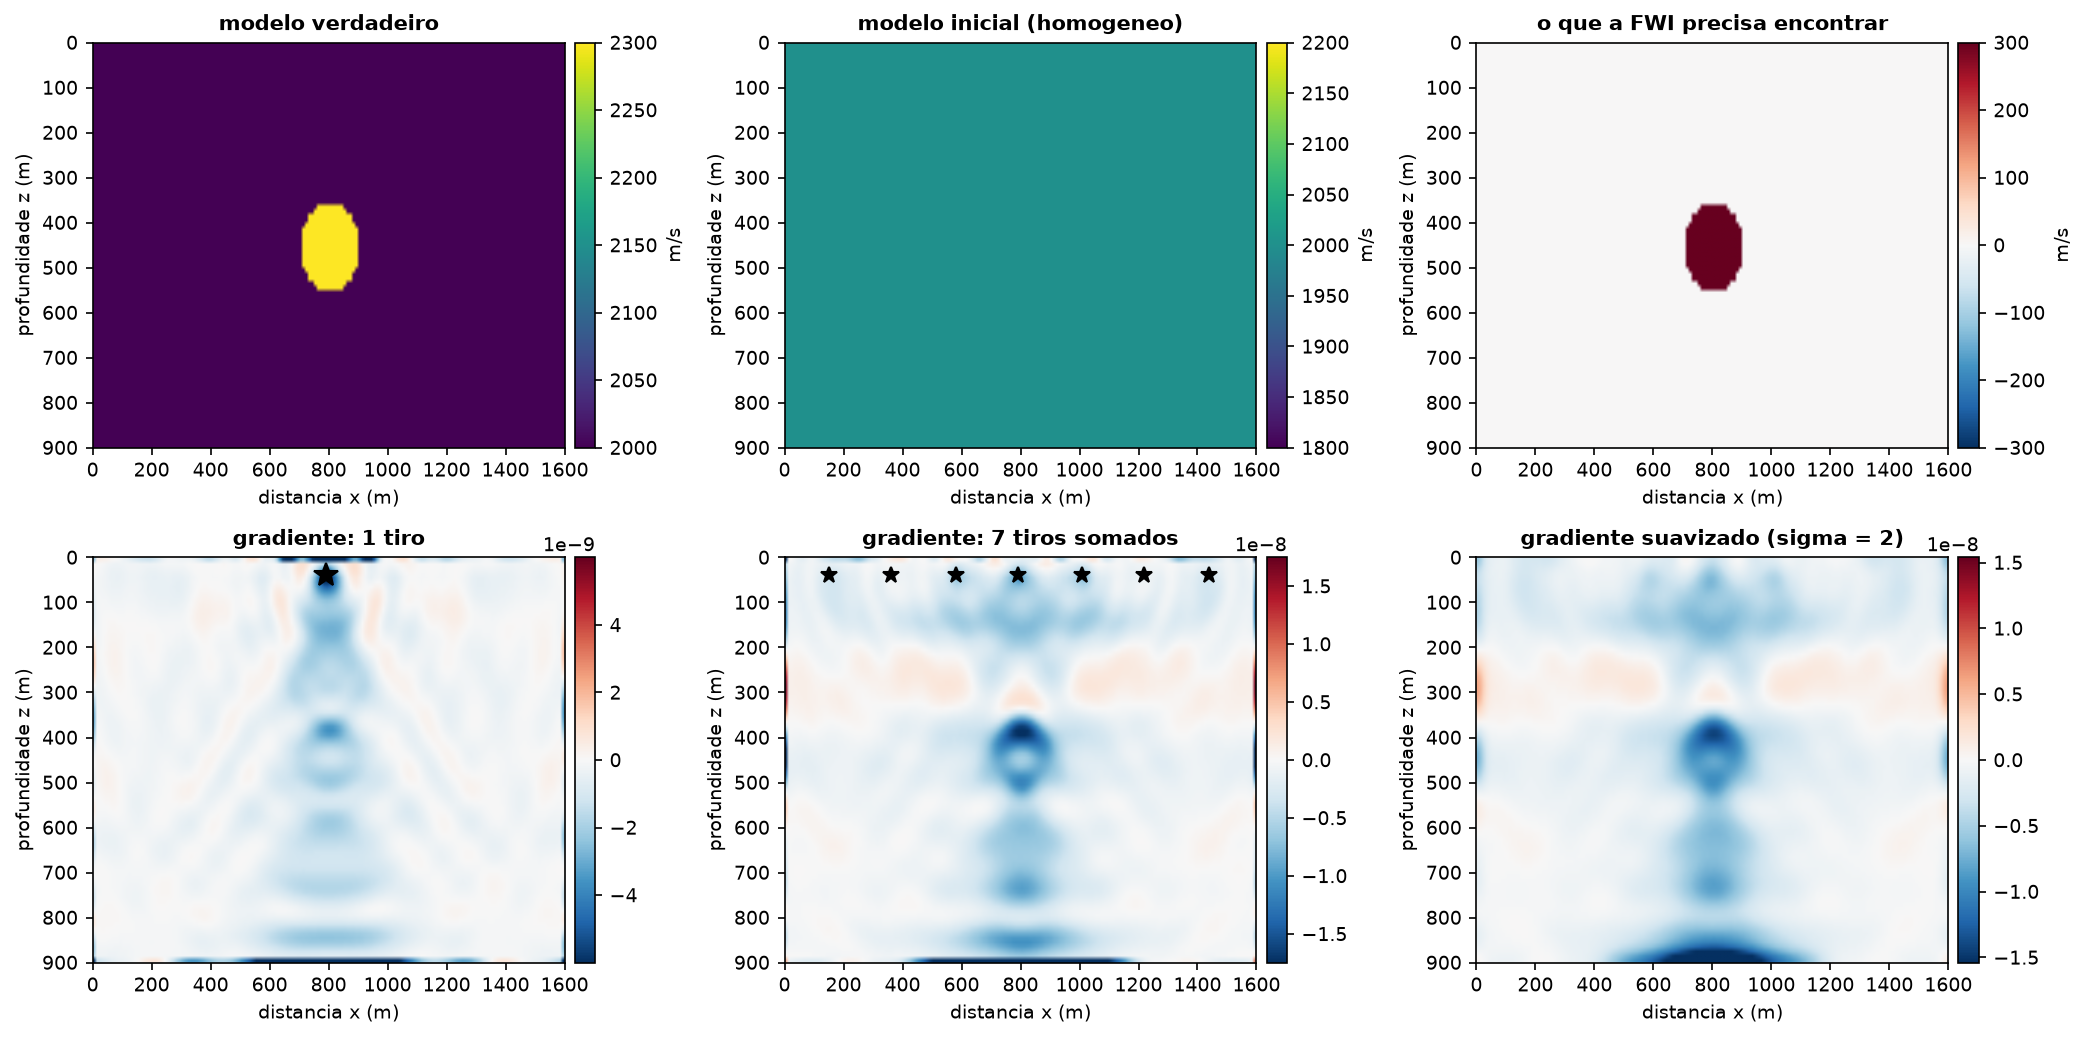
\includegraphics[width=0.96\textwidth]{../saidas/aula08/01_gradiente_adjunto.png}
\caption{Um gradiente de verdade, calculado pelo c\'odigo do curso: um \'unico
disparo (esquerda), sete disparos somados (centro) e o resultado suavizado
(direita). Um disparo isolado espalha a sensibilidade em arcos amb\'iguos; \'e
a \emph{soma} sobre disparos que localiza a anomalia.}
\end{figure}

Quatro coisas a observar em qualquer gradiente, sempre nesta ordem:

\begin{enumerate}[leftmargin=*]
\item \textbf{O sinal --- e em qual par\^ametro ele est\'a escrito.} A
atualiza\c{c}\~ao anda no sentido oposto ao gradiente, mas o sentido f\'isico
depende da vari\'avel. Em \textbf{velocidade}, gradiente negativo faz a
velocidade \emph{aumentar}. Em \textbf{vagarosidade ao quadrado} --- que \'e a
forma em que a f\'ormula sai naturalmente --- o sentido se \textbf{inverte},
porque $1/c^2$ diminui quando $c$ aumenta. Trocar os dois \'e um erro comum,
e produz uma invers\~ao que anda confiante na dire\c{c}\~ao errada. Confira
sempre contra uma perturba\c{c}\~ao conhecida.
\item \textbf{Artefato colado na fonte e nos receptores.} Ali o campo tem
amplitude enorme e a correla\c{c}\~ao explode. N\~ao \'e informa\c{c}\~ao
sobre a geologia: \'e geometria da aquisi\c{c}\~ao. Mascare.
\item \textbf{Os arcos.} Um par fonte--receptor n\~ao aponta um \emph{ponto}:
espalha a sensibilidade por uma faixa. Para ondas transmitidas essa faixa liga
a fonte ao receptor --- a ``banana''; para ondas refletidas, \'e um arco de
elipse com focos na fonte e no receptor. A espessura da faixa \'e a
\textbf{zona de Fresnel}: a onda \'e sens\'ivel a um \emph{volume}, n\~ao a um
ponto. A resolu\c{c}\~ao finita da FWI \'e consequ\^encia direta disso.
\item \textbf{A ilumina\c{c}\~ao cai com a profundidade.} A energia da onda se
espalha, e o gradiente \'e proporcional a ela. Medido com o c\'odigo deste
curso, a raz\~ao entre a sensibilidade rasa e a profunda chegou a
\textbf{181 vezes}. Sem corre\c{c}\~ao, a FWI s\'o atualiza a parte rasa do
modelo.
\end{enumerate}

\begin{pratica}[FWI e migra\c{c}\~ao s\~ao parentes pr\'oximos]
A f\'ormula do gradiente --- correlacionar o campo da fonte com o campo do
res\'iduo retropropagado --- \'e \emph{a mesma} condi\c{c}\~ao de imagem da
migra\c{c}\~ao reversa no tempo (RTM). Em ess\^encia, uma RTM \'e a primeira
itera\c{c}\~ao de uma FWI.

A diferen\c{c}a \'e o que se faz com o resultado: a migra\c{c}\~ao o trata
como uma \emph{imagem} das interfaces; a FWI o trata como uma
\emph{corre\c{c}\~ao} a ser aplicada ao modelo, e repete.
\end{pratica}

\begin{resumo}
\begin{itemize}[leftmargin=*, itemsep=1pt]
\item Gradiente = um n\'umero por c\'elula dizendo como $J$ reage a mexer
ali.
\item For\c{c}a bruta custa uma simula\c{c}\~ao por c\'elula: invi\'avel.
\item O estado adjunto obt\'em tudo com duas simula\c{c}\~oes por disparo ---
direta, e o res\'iduo reinjetado nos receptores rodando para tr\'as.
\item O gradiente \'e a correla\c{c}\~ao dos dois campos: grande onde ambos
passaram no mesmo instante.
\item Leia sempre: sinal, artefatos na aquisi\c{c}\~ao, arcos de Fresnel,
queda de ilumina\c{c}\~ao com a profundidade.
\end{itemize}
\end{resumo}

% =====================================================================
\chapter{Verifica\c{c}\~ao do gradiente}
\label{cap:verificacao}

\begin{ideia}
Um gradiente errado n\~ao trava o programa, n\~ao emite aviso e n\~ao produz
figura feia. Ele produz uma invers\~ao que roda at\'e o fim e devolve um
modelo plaus\'ivel e errado. Existe um teste barato que separa ``o c\'odigo
roda'' de ``o c\'odigo est\'a certo'', e este cap\'itulo \'e sobre ele.
\end{ideia}

\section{O modo de falha silencioso}

Vale insistir, porque \'e contraintuitivo: se voc\^e errar o gradiente ---
esquecer um fator, trocar um sinal, omitir um termo --- a FWI continua
funcionando \emph{aparentemente bem}. A curva de $J$ desce. O modelo final
tem estrutura. As figuras ficam apresent\'aveis.

\begin{armadilha}[Por que isso acontece]
Um gradiente errado geralmente ainda \'e uma dire\c{c}\~ao de descida
\emph{aproximada}: ele aponta mais ou menos para baixo, s\'o que torto. A
busca linear ent\~ao encontra um passo que reduz $J$, e o processo segue.

Voc\^e n\~ao descobre o erro pela execu\c{c}\~ao. Descobre quando algu\'em
tenta reproduzir, ou quando o resultado n\~ao bate com um po\c{c}o --- meses
depois.
\end{armadilha}

\section{A ideia do teste}

O gradiente \'e uma promessa sobre o que acontece com $J$ quando se anda um
pouquinho numa dire\c{c}\~ao. Basta cobrar a promessa: ande um pouquinho,
me\c{c}a $J$ de verdade, e compare com o que o gradiente previu.

Se a previs\~ao bate --- e bate \emph{cada vez melhor} conforme o passo
diminui --- o gradiente est\'a certo. Formalmente, os testes t\^em tr\^es
n\'iveis de rigor:

\begin{center}
\begin{tabular}{@{}lp{6.6cm}l@{}}
\toprule
\textbf{Teste} & \textbf{O que faz} & \textbf{Serve para} \\
\midrule
Pontual & compara c\'elula por c\'elula com a mexida bruta & \emph{localizar}
onde est\'a o erro \\
Direcional & compara a previs\~ao ao longo de uma dire\c{c}\~ao inteira, num
n\'umero s\'o & o teste do dia a dia \\
Taylor & verifica a \emph{taxa} com que o erro da previs\~ao encolhe & o
veredito final \\
\bottomrule
\end{tabular}
\end{center}

\begin{teoria}[O teste de Taylor, em palavras]
Se o gradiente estiver \textbf{certo}, ao reduzir o passo pela metade o erro
da previs\~ao cai por \textbf{quatro} --- porque o que sobra \'e s\'o a
curvatura, que \'e de segunda ordem.

Se o gradiente estiver \textbf{errado}, o erro cai apenas pela metade ---
porque sobrou um peda\c{c}o de primeira ordem que n\~ao deveria estar l\'a.

Essa diferen\c{c}a entre ``cai por 4'' e ``cai por 2'' \'e um sinal
inequ\'ivoco, e n\~ao depende de voc\^e saber a resposta certa de antem\~ao.
\end{teoria}

\begin{figure}[htbp]
\centering
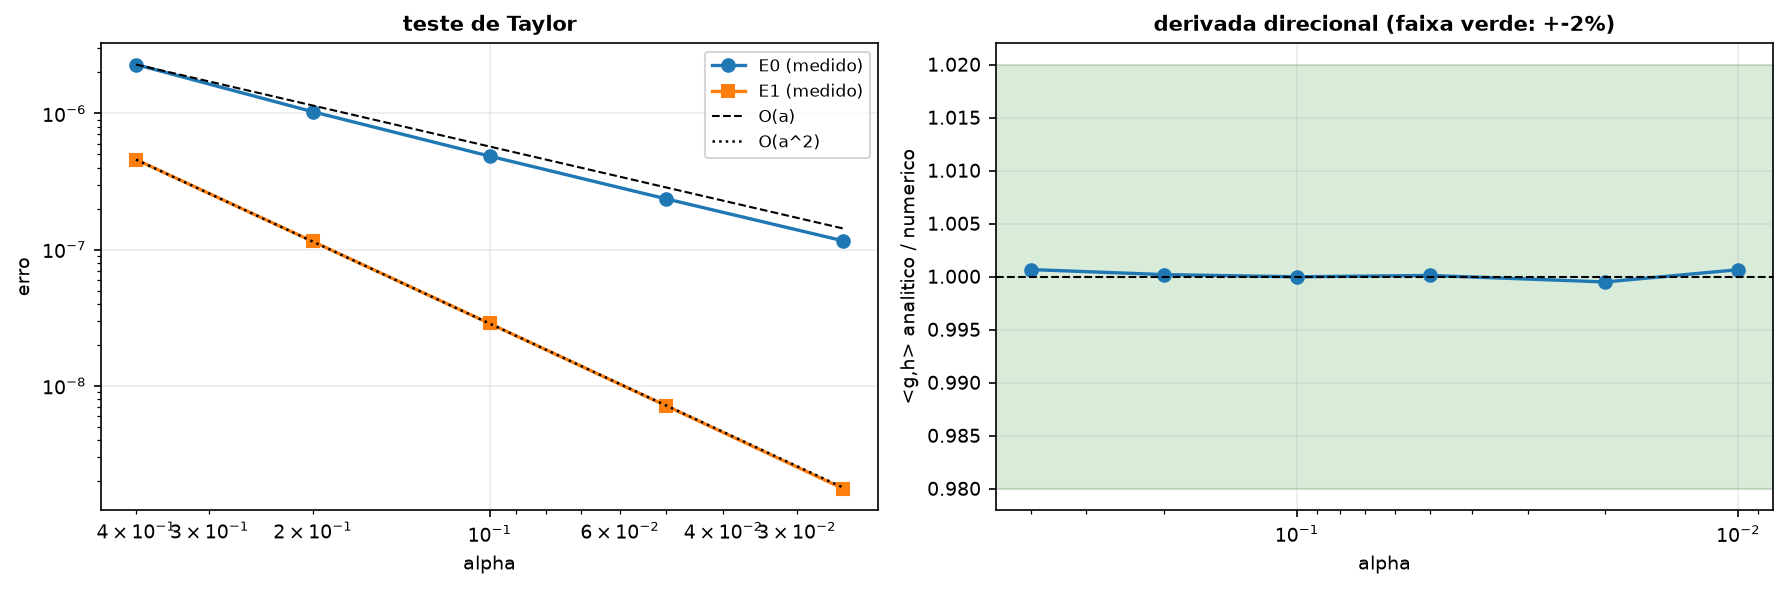
\includegraphics[width=0.96\textwidth]{../saidas/aula09/01_testes_de_gradiente.png}
\caption{Os testes rodados no propagador deste curso. \`A esquerda, em escala
logar\'itmica: a curva inferior deve ser paralela \`a refer\^encia de
inclina\c{c}\~ao 2. \`A direita, a raz\~ao entre previsto e medido, que deve
ficar em 1 --- e fica, dentro de $0{,}07\%$.}
\end{figure}

\section{Diagnosticar pelo padr\~ao}

O valor da raz\~ao entre previsto e medido n\~ao diz apenas ``passou'' ou
``n\~ao passou'' --- o \emph{padr\~ao} dela diz que tipo de erro voc\^e tem:

\begin{center}
\begin{tabular}{@{}p{4.4cm}p{10.4cm}@{}}
\toprule
\textbf{Padr\~ao observado} & \textbf{Diagn\'ostico} \\
\midrule
raz\~ao $\approx 1$, est\'avel & gradiente correto \\
raz\~ao est\'avel mas $\ne 1$ \newline (ex.: $0{,}91$ para todo passo)
  & erro \textbf{sistem\'atico}: fator de escala esquecido, sinal trocado,
    peso de quadratura faltando, ou um termo ausente. Valor est\'avel \'e boa
    not\'icia: o \emph{bug} \'e determin\'istico e localiz\'avel \\
raz\~ao inst\'avel, pulando & ru\'ido num\'erico: o passo est\'a pequeno demais
  para a precis\~ao usada. Aumente o passo ou use precis\~ao dupla \\
\bottomrule
\end{tabular}
\end{center}

\begin{pratica}[Um caso real, ocorrido na montagem deste curso]
O propagador \textbf{reprovou}: a raz\~ao dava $0{,}9118$ --- e dava
$0{,}9118$ para todos os tamanhos de passo, ao longo de uma faixa de 40 vezes.
Estabilidade perfeita: erro sistem\'atico.

O teste \emph{pontual} localizou a regi\~ao: raz\~ao $\approx 0{,}99$ no
miolo do modelo e $\approx 0{,}72$ perto da superf\'icie. O erro estava nas
bordas.

A causa: o modelo \'e \emph{estendido} com a moldura absorvente antes de
simular, replicando os pixels da borda. O gradiente voltava ao dom\'inio
f\'isico com um simples recorte --- jogando fora a sensibilidade acumulada
dentro da moldura, em vez de som\'a-la de volta sobre a borda que a gerou.

Corrigido, a raz\~ao passou de $0{,}9118$ para $1{,}0001$.
\end{pratica}

\begin{teoria}[A li\c{c}\~ao generaliz\'avel]
\textbf{Toda opera\c{c}\~ao aplicada ao modelo antes de simular precisa da sua
contrapartida no caminho de volta do gradiente}: extens\~ao de bordas,
interpola\c{c}\~ao entre malhas, suaviza\c{c}\~ao, mudan\c{c}a de
par\^ametro, mudan\c{c}a de unidade.

Esquecer uma delas produz exatamente o sintoma acima --- e o teste de
gradiente \'e o \'unico que acusa.
\end{teoria}

\begin{resumo}
\begin{itemize}[leftmargin=*, itemsep=1pt]
\item Gradiente errado \'e um erro \emph{silencioso}: a invers\~ao roda, $J$
cai, o modelo sai plaus\'ivel.
\item O teste \'e simples: ande um pouco, compare $J$ medido com $J$ previsto
pelo gradiente.
\item Gradiente certo $\Rightarrow$ ao dividir o passo por 2, o erro da
previs\~ao cai por 4. Gradiente errado $\Rightarrow$ cai s\'o por 2.
\item Raz\~ao est\'avel e diferente de 1 aponta \emph{bug} determin\'istico;
raz\~ao inst\'avel aponta ru\'ido num\'erico.
\item Nunca rode uma invers\~ao com um gradiente que n\~ao passou no teste.
\end{itemize}
\end{resumo}

% =====================================================================
\chapter{Otimiza\c{c}\~ao: escolher a dire\c{c}\~ao e o tamanho do passo}
\label{cap:otimizacao}

\begin{ideia}
O gradiente diz para que lado descer. Falta decidir \emph{exatamente} em que
dire\c{c}\~ao andar --- porque ``para baixo'' raramente \'e o caminho mais
curto --- e \emph{quanto} andar. Essas duas decis\~oes s\~ao onde o tempo de
m\'aquina \'e gasto.
\end{ideia}

\begin{matematica}[inclina\c{c}\~ao e curvatura]
Este cap\'itulo trata da diferen\c{c}a entre duas informa\c{c}\~oes sobre uma
paisagem.

\textbf{Inclina\c{c}\~ao} (o gradiente) diz \emph{para que lado} desce, e
nada mais. Ela \'e uma informa\c{c}\~ao puramente local: v\'alida no ponto
onde voc\^e est\'a, e s\'o.

\textbf{Curvatura} diz o qu\~ao r\'apido a inclina\c{c}\~ao muda quando
voc\^e anda --- ou seja, se o vale \`a sua frente \'e uma bacia larga e rasa
ou uma fenda estreita. Com essa informa\c{c}\~ao, d\'a para estimar
\emph{quanto} andar, e n\~ao s\'o para que lado.

A analogia que vale: descer uma montanha no nevoeiro. Sabendo s\'o a
inclina\c{c}\~ao, voc\^e d\'a passos curtos e cautelosos, e num desfiladeiro
acaba ricocheteando de parede em parede. Sabendo tamb\'em a curvatura, voc\^e
percebe que est\'a num corredor e passa a andar ao longo dele.

O objeto matem\'atico que guarda toda a curvatura chama-se \textbf{Hessiana}.
Em FWI ele \'e grande demais para existir --- com um milh\~ao de c\'elulas
seriam $10^{12}$ n\'umeros, v\'arios terabytes. Todo este cap\'itulo \'e sobre
como obter \emph{parte} dessa informa\c{c}\~ao de gra\c{c}a: ou acumulando o
hist\'orico dos \'ultimos passos, ou estimando a curvatura por um atalho
f\'isico (a ilumina\c{c}\~ao).
\end{matematica}

\section{Por que n\~ao basta seguir o gradiente}

Descer pela dire\c{c}\~ao de maior inclina\c{c}\~ao parece \'obvio, e \'e
ruim. Num vale alongado e estreito --- que \'e exatamente o formato de $J$ em
FWI --- a dire\c{c}\~ao de maior inclina\c{c}\~ao aponta para a
\emph{parede}, n\~ao para o fundo. O resultado \'e o ziguezague cl\'assico:

\begin{center}
\begin{tikzpicture}[scale=1.0]
% vale eliptico
\foreach \s in {0.5,1.0,1.5,2.0} {
  \draw[gray!35] (0,0) ellipse ({3.0*\s/2} and {0.62*\s/2});
}
\fill[verdefwi] (0,0) circle (0.08);
\node[font=\scriptsize, verdefwi, below=1pt] at (0,-0.12) {m\'inimo};
% ziguezague
\coordinate (p0) at (-2.7,0.42);
\draw[vermelhofwi, line width=1pt, -{Stealth[length=2mm]}]
  (-2.7,0.42) -- (-2.05,-0.30) -- (-1.35,0.25) -- (-0.85,-0.18)
  -- (-0.45,0.12) -- (-0.2,-0.07) -- (-0.05,0.03);
\fill[vermelhofwi] (-2.7,0.42) circle (0.07);
\node[font=\scriptsize, vermelhofwi, left=1pt] at (-2.75,0.42) {in\'icio};
\node[font=\scriptsize, vermelhofwi] at (-1.5,0.72) {descida m\'axima};
% direcao esperta
\draw[cianofwi, line width=1pt, dashed, -{Stealth[length=2mm]}]
  (-2.7,0.42) .. controls (-1.6,0.18) and (-0.8,0.06) .. (-0.06,0.01);
\node[font=\scriptsize, cianofwi] at (-1.3,-0.68) {m\'etodo com mem\'oria};
\end{tikzpicture}
\end{center}

Os m\'etodos melhores usam \textbf{mem\'oria}: olham para os passos
anteriores e deduzem em que dire\c{c}\~ao o vale se estende.

\begin{center}
\begin{tabular}{@{}llp{6.3cm}@{}}
\toprule
\textbf{M\'etodo} & \textbf{Usa} & \textbf{Em FWI} \\
\midrule
Descida m\'axima & s\'o o gradiente atual & barato e lento; ziguezagueia \\
Gradiente conjugado & gradiente + dire\c{c}\~ao anterior & bom custo/benef\'icio,
mem\'oria m\'inima \\
l-BFGS & os \'ultimos $\sim$5--20 passos & \textbf{o padr\~ao} da \'area:
reconstr\'oi a forma do vale a partir do hist\'orico \\
Newton & a curvatura exata (Hessiana) & imposs\'ivel: a matriz teria
$10^{12}$ entradas \\
\bottomrule
\end{tabular}
\end{center}

Medindo num problema real de FWI com o c\'odigo do curso (12 itera\c{c}\~oes,
mesmo pr\'e-condicionamento, erro do modelo inicial de $4{,}71\%$):

\begin{center}
\begin{tabular}{@{}lrrr@{}}
\toprule
\textbf{M\'etodo} & $J_{\text{final}}/J_0$ & \textbf{erro final}
& \textbf{simula\c{c}\~oes gastas} \\
\midrule
Descida m\'axima    & $0{,}1035$ & $3{,}82\%$ & 30 \\
Gradiente conjugado & $0{,}0493$ & $3{,}29\%$ & 28 \\
l-BFGS              & $0{,}0419$ & $3{,}26\%$ & 28 \\
\bottomrule
\end{tabular}
\end{center}

\begin{atencao}[Compare por custo, n\~ao por itera\c{c}\~ao]
Por \emph{itera\c{c}\~ao}, o l-BFGS quase sempre vence. Mas cada itera\c{c}\~ao
pode custar mais tentativas de passo --- e o que consome tempo de m\'aquina
\'e o n\'umero de \textbf{simula\c{c}\~oes}, n\~ao o n\'umero de
itera\c{c}\~oes.

Sempre que comparar otimizadores num relat\'orio, mostre o eixo de custo.
Comparar por itera\c{c}\~ao favorece artificialmente os m\'etodos de
itera\c{c}\~ao cara.
\end{atencao}

\section{Quanto andar: a busca linear}

Escolhida a dire\c{c}\~ao, resta o tamanho do passo. Passo pequeno demais
desperdi\c{c}a itera\c{c}\~oes; grande demais pode piorar $J$ --- ou empurrar
a velocidade para valores absurdos, violar a condi\c{c}\~ao CFL do
Cap\'itulo~\ref{cap:numerico} e fazer a simula\c{c}\~ao explodir.

O procedimento padr\~ao \'e tentar um passo, avaliar $J$, e ajustar. Cada
tentativa custa \textbf{uma simula\c{c}\~ao completa de todos os disparos} ---
por isso a busca linear \'e frequentemente mais cara que o pr\'oprio
gradiente.

\begin{pratica}[O chute inicial que funciona]
Em FWI, o crit\'erio com significado f\'isico \'e simples: \textbf{n\~ao
altere o modelo em mais de 1\% a 3\% de uma vez}. Isso \'e mais confi\'avel
que qualquer estimativa puramente matem\'atica, porque respeita a escala do
problema.
\end{pratica}

\section{A ilumina\c{c}\~ao desigual e o pr\'e-condicionamento}

Existe um problema mais sutil que a dire\c{c}\~ao: o gradiente \'e
sistematicamente \textbf{maior perto da superf\'icie}, simplesmente porque a
onda \'e mais intensa ali. Sem corre\c{c}\~ao, o algoritmo gasta toda a
atualiza\c{c}\~ao no raso e n\~ao toca no profundo.

A corre\c{c}\~ao chama-se \textbf{pr\'e-condicionamento}: dividir o gradiente
por uma estimativa da ilumina\c{c}\~ao de cada ponto --- essencialmente, pela
energia do campo de onda ali.

\begin{teoria}[Isso n\~ao \'e cosm\'etico]
Dividir pela ilumina\c{c}\~ao parece um truque para a figura ficar bonita, e
n\~ao \'e. \'E uma aproxima\c{c}\~ao barata e justificada da corre\c{c}\~ao de
curvatura que o m\'etodo de Newton faria, se a Hessiana pudesse ser montada.
Tem nome na literatura (\emph{pseudo-Hessiano}) e refer\^encia.

O que ele \textbf{n\~ao} faz: n\~ao corrige \emph{cycle skipping}, n\~ao
inventa informa\c{c}\~ao onde n\~ao houve ilumina\c{c}\~ao, e n\~ao substitui
um bom modelo inicial.
\end{teoria}

Efeito medido no curso (correla\c{c}\~ao do gradiente com a perturba\c{c}\~ao
verdadeira):

\begin{center}
\begin{tabular}{@{}lr@{}}
\toprule
\textbf{Vers\~ao do gradiente} & \textbf{Correla\c{c}\~ao} \\
\midrule
bruto & $+0{,}0390$ \\
mascarado na faixa de fonte/receptor & $+0{,}0830$ \\
mascarado + suavizado & $+0{,}0842$ \\
+ compensa\c{c}\~ao de profundidade & $+0{,}0898$ \\
\bottomrule
\end{tabular}
\end{center}

\begin{atencao}[Como ler esses n\'umeros]
Os valores absolutos s\~ao baixos, e isso est\'a \emph{certo}: um gradiente
n\~ao \'e o modelo, \'e uma dire\c{c}\~ao de busca espalhada em arcos de
Fresnel. Esperar correla\c{c}\~ao alta seria esperar que a FWI terminasse numa
itera\c{c}\~ao.

O que importa \'e a varia\c{c}\~ao \emph{relativa}: o tratamento
\textbf{mais que dobra} a correla\c{c}\~ao, e esse ganho, repetido a cada
itera\c{c}\~ao, muda a converg\^encia da invers\~ao inteira.
\end{atencao}

\textbf{Receita, em ordem de import\^ancia:} (1) mascare a faixa de
fonte/receptor; (2) compense a ilumina\c{c}\~ao; (3) suavize levemente;
(4) mantenha o modelo dentro de uma caixa de velocidades fisicamente
plaus\'iveis.

\begin{resumo}
\begin{itemize}[leftmargin=*, itemsep=1pt]
\item Seguir s\'o o gradiente ziguezagueia; m\'etodos com mem\'oria (CG,
l-BFGS) seguem o eixo do vale.
\item O tamanho do passo \'e escolhido por tentativa, e cada tentativa custa
uma simula\c{c}\~ao completa.
\item Compare otimizadores por \emph{custo}, n\~ao por itera\c{c}\~ao.
\item O gradiente bruto \'e dominado pelo raso; pr\'e-condicionar pela
ilumina\c{c}\~ao \'e uma aproxima\c{c}\~ao justificada de Newton, n\~ao
maquiagem.
\end{itemize}
\end{resumo}

% =====================================================================
\chapter{A FWI completa: o fluxo de trabalho}
\label{cap:completa}

\begin{ideia}
Juntando as pe\c{c}as: prepare o dado, escolha um modelo inicial, suba as
frequ\^encias em degraus, e --- a parte que mais se esquece --- \emph{prove}
que o resultado \'e melhor do que o ponto de partida.
\end{ideia}

\section{O fluxo, do come\c{c}o ao fim}

\begin{center}
\begin{tikzpicture}[node distance=5mm,
  et/.style={draw, rounded corners=3pt, line width=0.9pt, align=left,
             text width=10.3cm, font=\small, inner sep=6pt},
  seta/.style={-{Stealth[length=2.4mm]}, line width=0.9pt, gray!60}]
\node[et, draw=azulfwi, fill=azulfwi!5] (e1)
  {\textbf{1. Preparar o dado.} Remover a onda direta se n\~ao for modelada;
   decidir o que fazer com as m\'ultiplas; estimar a ondaleta da fonte.};
\node[et, draw=cianofwi, fill=cianofwi!5, below=of e1] (e2)
  {\textbf{2. Modelo inicial.} Tomografia, an\'alise de velocidade, po\c{c}os.
   Precisa acertar as escalas grandes, n\~ao os detalhes.};
\node[et, draw=roxofwi, fill=roxofwi!5, below=of e2] (e3)
  {\textbf{3. Dimensionar a simula\c{c}\~ao.} $\Delta h$, $\Delta t$, moldura
   absorvente --- Cap.~\ref{cap:numerico} e \ref{cap:bordas}.};
\node[et, draw=verdefwi, fill=verdefwi!5, below=of e3] (e4)
  {\textbf{4. Verificar o gradiente.} Antes da primeira invers\~ao, n\~ao
   depois --- Cap.~\ref{cap:verificacao}.};
\node[et, draw=amarelofwi, fill=amarelofwi!8, below=of e4] (e5)
  {\textbf{5. Multiescala.} Para cada banda, do baixo para o alto: filtrar o
   dado, rodar algumas itera\c{c}\~oes, passar o modelo adiante.};
\node[et, draw=vermelhofwi, fill=vermelhofwi!5, below=of e5] (e6)
  {\textbf{6. Diagnosticar e reportar.} Perfis, mapa de erro, curva de
   converg\^encia, res\'iduo final --- e sempre o erro do modelo
   \emph{inicial}.};
\foreach \a/\b in {e1/e2, e2/e3, e3/e4, e4/e5, e5/e6} \draw[seta] (\a) -- (\b);
\end{tikzpicture}
\end{center}

\section{Um experimento controlado}

O c\'odigo do curso comparou monoescala (direto em 25\,Hz) contra multiescala
(5, depois 12, depois 25\,Hz), com \emph{o mesmo n\'umero total de
itera\c{c}\~oes} --- a \'unica diferen\c{c}a sendo a ordem em que a
informa\c{c}\~ao entra:

\begin{center}
\begin{tabular}{@{}lrrr@{}}
\toprule
\textbf{M\'etrica} & \textbf{Inicial} & \textbf{Mono (25\,Hz)}
& \textbf{Multi (5/12/25)} \\
\midrule
Erro relativo do modelo & $8{,}00\%$ & $7{,}35\%$ & $\mathbf{7{,}20\%}$ \\
Ganho sobre o inicial & --- & $+8{,}1\%$ & $+10{,}0\%$ \\
Tempo & --- & 3{,}8 min & 5{,}7 min \\
\bottomrule
\end{tabular}
\end{center}

\begin{atencao}[Leia este resultado com honestidade]
A vantagem da multiescala aqui \'e real mas \textbf{modesta}. E isso \'e
esperado: o modelo inicial tem apenas 8\% de erro, ou seja, j\'a est\'a
\emph{dentro} do vale de atra\c{c}\~ao de 25\,Hz. Quando o monoescala n\~ao
sofre \emph{cycle skipping}, n\~ao h\'a muito para a multiescala resgatar.

A honestidade aqui n\~ao \'e detalhe de estilo: um experimento que confirma o
que voc\^e queria, pelo motivo errado, \'e pior que nenhum experimento.
\end{atencao}

\section{O fracasso que n\~ao parece fracasso}

O estudo de robustez do curso degradou o modelo inicial de prop\'osito. Um dos
casos merece aten\c{c}\~ao especial:

\begin{center}
\begin{tabular}{@{}lrrr@{}}
\toprule
\textbf{Modelo inicial} & \textbf{erro inicial} & \textbf{mono 25\,Hz}
& \textbf{multi 5/12/25} \\
\midrule
linear suave              & $7{,}96\%$  & $7{,}34\%$  & $\mathbf{7{,}07\%}$ \\
\textbf{linear lento (viesado)} & $\mathbf{16{,}68\%}$ & $\mathbf{17{,}57\%}$
  & $\mathbf{17{,}34\%}$ \\
constante                 & $16{,}32\%$ & $16{,}10\%$ & $16{,}06\%$ \\
suavizado forte           & $4{,}95\%$  & $4{,}01\%$  & $\mathbf{3{,}70\%}$ \\
\bottomrule
\end{tabular}
\end{center}

\begin{armadilha}[Olhe a segunda linha]
O erro inicial era $16{,}68\%$ e a FWI terminou em $17{,}57\%$. Ou seja: a
invers\~ao \textbf{piorou o modelo}.

Ela n\~ao travou, n\~ao emitiu erro, e a fun\c{c}\~ao objetivo caiu
direitinho. Ela simplesmente convergiu para um m\'inimo local e, no caminho,
degradou o que j\'a se sabia.

Este \'e o fracasso mais perigoso da FWI, porque \emph{n\~ao se parece com
fracasso}. Olhando s\'o a curva de $J$ e a figura do modelo final, voc\^e
concluiria que funcionou.
\end{armadilha}

Repare tamb\'em na quarta linha: o \emph{melhor} resultado absoluto
($3{,}70\%$) veio do modelo inicial mais privilegiado. Compare com o inicial
constante, que termina em $16\%$. \textbf{A diferen\c{c}a entre os dois n\~ao
est\'a no algoritmo --- est\'a no que j\'a se sabia antes de come\c{c}ar.}

\section{Como reportar uma FWI}

\begin{teoria}[O m\'inimo que sustenta uma conclus\~ao]
Uma figura de ``antes e depois'' n\~ao sustenta nada. Reporte:
\begin{itemize}[leftmargin=*, itemsep=1pt]
\item \textbf{erro relativo do modelo}, comparado com o do modelo inicial;
\item \textbf{curva de converg\^encia} de $J$, com eixo de \emph{custo};
\item \textbf{perfis verticais} comparando verdadeiro, inicial e invertido;
\item \textbf{mapa de erro}, que revela \emph{onde} o m\'etodo falhou;
\item \textbf{compara\c{c}\~ao de sismogramas} observado contra final.
\end{itemize}

E a exig\^encia central: \textbf{relate o erro do modelo inicial}. Uma FWI que
vai de 2\% para $1{,}5\%$ n\~ao demonstra quase nada; uma que vai de 20\% para
5\% demonstra muito. Sem o ponto de partida, o n\'umero final n\~ao significa
nada.
\end{teoria}

\begin{figure}[htbp]
\centering
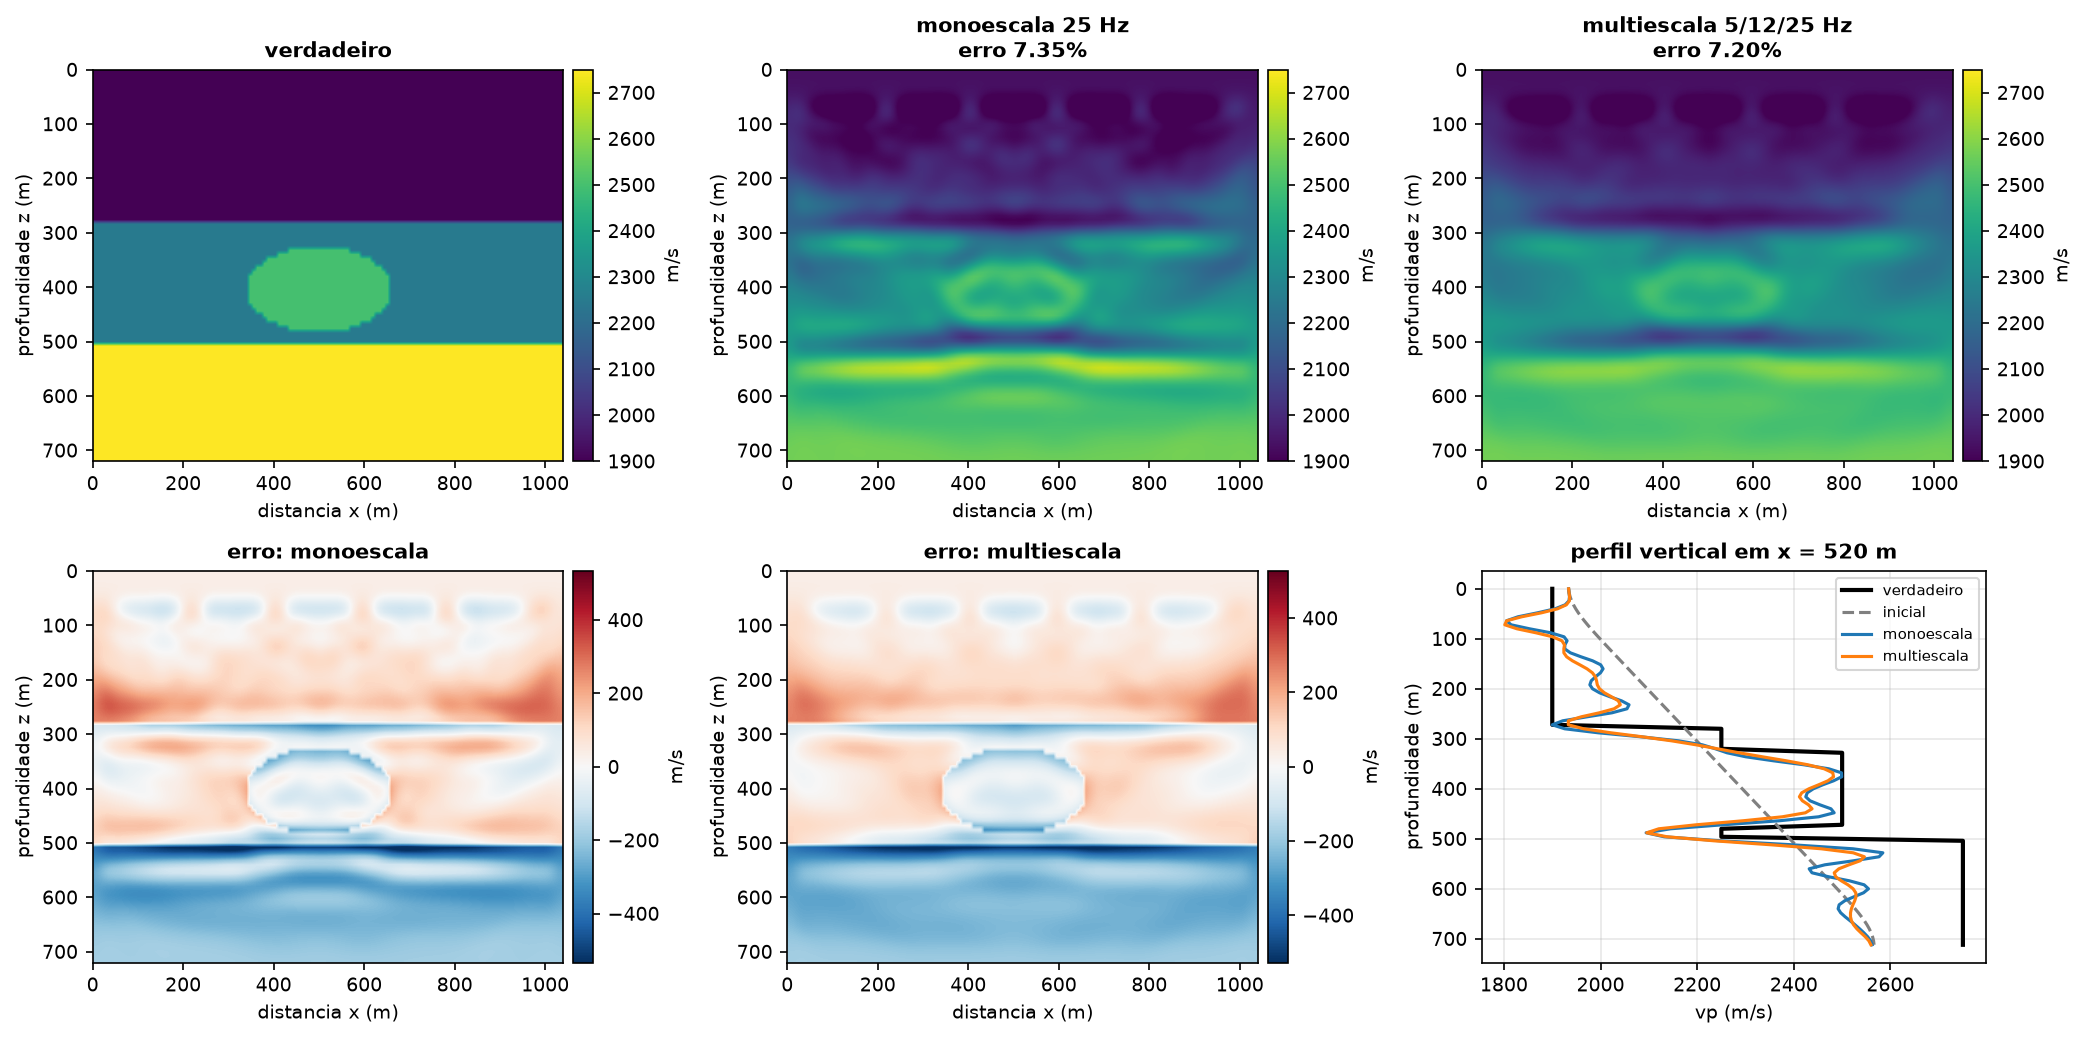
\includegraphics[width=0.96\textwidth]{../saidas/aula12/02_mono_vs_multi.png}
\caption{Monoescala \emph{versus} multiescala: modelos recuperados, mapas de
erro e perfil vertical. O mapa de erro \'e a figura mais informativa das
tr\^es --- ele mostra \emph{onde} a invers\~ao n\~ao chegou.}
\end{figure}

\begin{resumo}
\begin{itemize}[leftmargin=*, itemsep=1pt]
\item O fluxo: preparar dado, modelo inicial, dimensionar, \emph{verificar
gradiente}, multiescala, diagnosticar.
\item A vantagem da multiescala s\'o aparece quando o monoescala sofreria
\emph{cycle skipping}.
\item Uma FWI pode \textbf{piorar} o modelo, com $J$ caindo o tempo todo. Sem
comparar com o inicial, voc\^e n\~ao percebe.
\item Reportar sem o erro do modelo inicial \'e reportar nada.
\end{itemize}
\end{resumo}

% =====================================================================
\chapter{Regulariza\c{c}\~ao e informa\c{c}\~ao a priori}
\label{cap:regularizacao}

\begin{ideia}
Existem partes do modelo que o dado simplesmente n\~ao enxerga. Ali o
algoritmo est\'a livre para inventar. Regularizar \'e dizer, de antem\~ao, que
tipo de invento voc\^e aceita.
\end{ideia}

\section{Por que o dado n\~ao basta}

A FWI \'e \textbf{mal posta} em dois sentidos, e vale distingui-los:

\begin{itemize}[leftmargin=*]
\item \textbf{Espa\c{c}o nulo.} Existem mudan\c{c}as no modelo que praticamente
n\~ao alteram o dado: regi\~oes n\~ao iluminadas, detalhes menores que meio
comprimento de onda, combina\c{c}\~oes de par\^ametros cujos efeitos se
cancelam. O dado \'e \emph{indiferente} a elas.
\item \textbf{Amplifica\c{c}\~ao de ru\'ido.} Nas dire\c{c}\~oes em que a
sensibilidade \'e baixa, um res\'iduo pequeno --- que pode ser s\'o ru\'ido
--- exige uma mudan\c{c}a \emph{grande} no modelo para ser explicado. O
resultado \'e estrutura de alta amplitude sem nenhum apoio nos dados.
\end{itemize}

A resposta padr\~ao \'e somar ao funcional um termo que penaliza modelos
indesej\'aveis:
\begin{equation}
J_{\text{total}} = \underbrace{J_{\text{dados}}}_{\text{ajustar o dado}}
 \;+\; \lambda\,\underbrace{R(\mvec)}_{\text{parecer plaus\'ivel}}
\end{equation}
com $\lambda$ regulando o peso relativo das duas exig\^encias.

\begin{atencao}[Uma distin\c{c}\~ao que evita confus\~ao]
Regulariza\c{c}\~ao \textbf{n\~ao} melhora o ajuste dos dados. Por
constru\c{c}\~ao, no \'otimo, $J_{\text{dados}}$ s\'o pode ficar igual ou
\emph{pior} do que ficaria sem ela.

O que ela faz \'e \emph{escolher}, entre os muitos modelos que ajustam os
dados praticamente igual, aquele que \'e mais plaus\'ivel segundo um
crit\'erio que \textbf{voc\^e} definiu. Isso significa que a escolha de $R$ \'e
uma afirma\c{c}\~ao sobre a geologia, e deve ser justificada como tal.
\end{atencao}

\begin{matematica}[somar quadrados ou somar m\'odulos: por que a escolha muda o resultado]
Os dois penalizadores a seguir medem ``o quanto o modelo varia'' --- e diferem
em uma \'unica coisa: se os desn\'iveis entram ao quadrado ou em m\'odulo.
Essa \'unica diferen\c{c}a muda o tipo de geologia que sai no fim.

Imagine dez degraus de $0{,}1$ cada, ou um \'unico degrau de $1$. A
varia\c{c}\~ao total \'e a mesma nos dois casos.

\textbf{Somando m\'odulos} ($L_1$): $10\times0{,}1 = 1$ contra $1$. Empate ---
os dois custam o mesmo.

\textbf{Somando quadrados} ($L_2$): $10\times(0{,}1)^{2} = 0{,}1$ contra
$1^{2} = 1$. O degrau \'unico custa \textbf{dez vezes mais}.

A consequ\^encia \'e direta: uma penalidade que usa quadrados \emph{detesta}
saltos e prefere rampas --- ou seja, \textbf{borra interfaces}. Uma que usa
m\'odulos \'e indiferente entre as duas formas de acomodar a varia\c{c}\~ao, e
por isso \textbf{tolera interfaces n\'itidas} enquanto ainda pune
oscila\c{c}\~ao dispersa.

Nenhuma das duas \'e ``mais correta''. Cada uma \'e uma afirma\c{c}\~ao
diferente sobre como voc\^e acredita que a subsuperf\'icie seja.
\end{matematica}

\section{Os dois penalizadores cl\'assicos}

\begin{center}
\begin{tikzpicture}[scale=1.0]
% Tikhonov
\node[font=\small\bfseries, azulfwi] at (2.3,2.5) {Tikhonov: prefere suave};
\draw[gray!45] (0,0) -- (4.6,0);
\draw[azulfwi, line width=1.2pt] (0,0.35) .. controls (1.6,0.35) and (2.0,1.75)
  .. (4.6,1.75);
\draw[gray!55, dashed, line width=0.7pt] (0,0.35) -- (2.3,0.35) -- (2.3,1.75)
  -- (4.6,1.75);
\node[font=\scriptsize, gray!70] at (3.5,0.6) {(verdade)};
% TV
\begin{scope}[xshift=6.6cm]
\node[font=\small\bfseries, verdefwi] at (2.3,2.5) {Varia\c{c}\~ao Total:
  prefere degraus};
\draw[gray!45] (0,0) -- (4.6,0);
\draw[verdefwi, line width=1.2pt] (0,0.35) -- (2.3,0.35) -- (2.3,1.75)
  -- (4.6,1.75);
\draw[gray!55, dashed, line width=0.7pt] (0,0.35) -- (2.3,0.35) -- (2.3,1.75)
  -- (4.6,1.75);
\end{scope}
\end{tikzpicture}
\end{center}

\begin{itemize}[leftmargin=*]
\item \textbf{Tikhonov} penaliza o \emph{quadrado} da varia\c{c}\~ao espacial.
Para ela, uma varia\c{c}\~ao grande e concentrada \'e muito mais cara do que a
mesma varia\c{c}\~ao dilu\'ida em muitos passinhos. Resultado: ela
\textbf{suaviza}, e borra as interfaces.
\item \textbf{Varia\c{c}\~ao Total (TV)} penaliza a varia\c{c}\~ao
\emph{total}, sem elevar ao quadrado. Um degrau grande e cem degrauzinhos
custam o mesmo. Resultado: ela pune a oscila\c{c}\~ao de ru\'ido, mas
\textbf{preserva interfaces n\'itidas}.
\end{itemize}

A tabela abaixo \'e a conta que explica a diferen\c{c}a inteira --- o custo de
acomodar uma varia\c{c}\~ao total de 1:

\begin{center}
\begin{tabular}{@{}lrr@{}}
\toprule
 & \textbf{Tikhonov} & \textbf{TV} \\
\midrule
um salto de 1 em um \'unico ponto & $1{,}00$ & $1{,}00$ \\
a mesma varia\c{c}\~ao em 10 passos de $0{,}1$ & $\mathbf{0{,}10}$ & $1{,}00$ \\
\bottomrule
\end{tabular}
\end{center}

\textbf{Escolha:} alvo estratificado com contatos n\'itidos pede TV;
varia\c{c}\~ao gradual pede Tikhonov.

\section{Um resultado que contraria a expectativa}

O experimento do curso usou dado com ru\'ido de mesma energia que o sinal
(rela\c{c}\~ao sinal/ru\'ido de 0\,dB) --- condi\c{c}\~ao dura, em que a
regulariza\c{c}\~ao deveria brilhar:

\begin{center}
\begin{tabular}{@{}lr@{}}
\toprule
\textbf{Variante} & \textbf{Erro final} \\
\midrule
modelo inicial & $4{,}75\%$ \\
sem regulariza\c{c}\~ao & $3{,}60\%$ \\
com Tikhonov & $4{,}42\%$ \\
com TV & $4{,}39\%$ \\
\textbf{apenas suavizando o gradiente} & $\mathbf{3{,}56\%}$ \\
\bottomrule
\end{tabular}
\end{center}

A regulariza\c{c}\~ao expl\'icita \textbf{piorou} o resultado, e o melhor
resultado veio da opera\c{c}\~ao mais simples da tabela.

\begin{teoria}[Por que ela perdeu aqui --- e a li\c{c}\~ao geral]
O modelo inicial j\'a era suave, e com poucas itera\c{c}\~oes a invers\~ao
n\~ao teve tempo de gerar rugosidade. O erro que sobrava \textbf{n\~ao era
rugosidade}: era falta de \emph{contraste} --- os degraus de velocidade ainda
n\~ao tinham sido recuperados em amplitude.

Tikhonov e TV penalizam exatamente a varia\c{c}\~ao espacial, isto \'e,
penalizam o contraste que ainda faltava construir. Estavam puxando na
dire\c{c}\~ao errada \emph{para este problema}.

\textbf{A li\c{c}\~ao:} diagnostique antes de escolher $R$. Se o erro residual
\'e rugosidade, Tikhonov e TV ajudam. Se \'e falta de contraste ou de
resolu\c{c}\~ao, atrapalham.
\end{teoria}

\begin{pratica}[A regulariza\c{c}\~ao que voc\^e j\'a est\'a usando sem saber]
Boa parte da FWI \'e regularizada implicitamente, e raramente isso \'e
reconhecido:
\begin{itemize}[leftmargin=*, itemsep=1pt]
\item suavizar o gradiente a cada itera\c{c}\~ao;
\item come\c{c}ar de um modelo inicial suave --- ele j\'a restringe onde a
solu\c{c}\~ao pode chegar;
\item a pr\'opria estrat\'egia multiescala: as bandas baixas imp\~oem
suavidade;
\item parar cedo: poucas itera\c{c}\~oes n\~ao produzem alta frequ\^encia;
\item limitar o modelo a uma caixa de velocidades.
\end{itemize}

Somar regulariza\c{c}\~ao expl\'icita a tudo isso frequentemente
\textbf{sobre-regulariza}. O sintoma \'e o da tabela acima: o modelo fica mais
suave e o erro \emph{aumenta}.
\end{pratica}

\section{Escolhendo o peso, e os v\'inculos que valem sempre}

\textbf{Como calibrar $\lambda$.} Escolha-o de modo que $\lambda R$ valha uma
fra\c{c}\~ao conhecida de $J_{\text{dados}}$ no ponto inicial --- 2\%, por
exemplo. Isso torna a escolha independente de unidades e reprodut\'ivel, muito
melhor que testar pot\^encias de 10 \`as cegas. Depois, refine pela
\textbf{curva em L}: varie $\lambda$, ponha o ajuste dos dados num eixo e a
penalidade no outro, e escolha o \emph{cotovelo} da curva.

\begin{armadilha}[Uma exig\^encia de honestidade]
Em problema sint\'etico voc\^e conhece o modelo verdadeiro e poderia escolher
$\lambda$ pelo menor erro de modelo. Em dado \textbf{real} isso \'e
imposs\'ivel --- voc\^e s\'o tem o ajuste e a penalidade. \'E para isso que
existe a curva em L.

Se voc\^e reportar resultados escolhendo $\lambda$ pelo erro de modelo, diga
isso explicitamente; caso contr\'ario o resultado parece melhor do que seria
na pr\'atica.
\end{armadilha}

\begin{center}
\begin{tabular}{@{}lll@{}}
\toprule
\textbf{V\'inculo} & \textbf{Como} & \textbf{Quando} \\
\midrule
Caixa de velocidades & cortar em $v_{\min}, v_{\max}$ ap\'os cada passo
  & \textbf{sempre} \\
\'Agua fixa & zerar o gradiente na l\^amina d'\'agua & dado marinho \\
M\'ascara de profundidade & zerar abaixo da penetra\c{c}\~ao & evita
  artefato \\
Modelo a priori & penalizar o afastamento do que se sabe & h\'a po\c{c}o ou
  tomografia \\
Rela\c{c}\~ao entre par\^ametros & amarrar $v_s$ e $\rho$ a $v_p$ &
  multipar\^ametro \\
\bottomrule
\end{tabular}
\end{center}

A caixa de velocidades parece grosseira, mas evita o modo de falha mais comum
da FWI: um passo ruim empurra a velocidade para um valor n\~ao f\'isico, a
simula\c{c}\~ao viola a condi\c{c}\~ao CFL e a invers\~ao n\~ao se recupera.

\begin{resumo}
\begin{itemize}[leftmargin=*, itemsep=1pt]
\item H\'a partes do modelo que o dado n\~ao restringe; regularizar \'e
escolher o que preencher ali.
\item Regularizar nunca melhora o ajuste dos dados --- escolhe entre modelos
que ajustam igual.
\item Tikhonov suaviza; TV preserva degraus. A escolha \'e uma afirma\c{c}\~ao
sobre a geologia.
\item Diagnostique o erro antes de escolher: rugosidade pede
regulariza\c{c}\~ao, falta de contraste n\~ao.
\item Suavizar o gradiente, parar cedo e come\c{c}ar suave j\'a s\~ao
regulariza\c{c}\~ao. Somar mais frequentemente sobre-regulariza.
\end{itemize}
\end{resumo}

% =====================================================================
\part*{\centering\color{azulfwi} Parte III --- Os limites}
\addcontentsline{toc}{part}{Parte III --- Os limites}

\chapter{Os limites da f\'isica adotada}
\label{cap:limites}

\begin{ideia}
Toda a cole\c{c}\~ao usou uma f\'isica simplificada. Este cap\'itulo
apresenta a fatura: o que cada simplifica\c{c}\~ao custa, como o custo
aparece no resultado, e como decidir se vale a pena pagar por f\'isica melhor.
\end{ideia}

\section{O invent\'ario de hip\'oteses}

\begin{center}
\begin{tabular}{@{}lll@{}}
\toprule
\textbf{Hip\'otese} & \textbf{Onde entrou} & \textbf{Quando quebra} \\
\midrule
sem cisalhamento ($\mu=0$) & Cap.~\ref{cap:fisica} & terrestre, contrastes de
  $v_s$ \\
densidade constante & Cap.~\ref{cap:fisica} & contrastes de imped\^ancia \\
sem atenua\c{c}\~ao & Cap.~\ref{cap:fisica} & meio dissipativo, banda larga \\
isotropia & Cap.~\ref{cap:fisica} & folhelhos, fraturas \\
2D & cole\c{c}\~ao inteira & estrutura fora do plano \\
fonte conhecida & Cap.~\ref{cap:bordas} & dado real: a ondaleta \'e estimada \\
ru\'ido aleat\'orio & Cap.~\ref{cap:misfit} & ru\'ido coerente, m\'ultiplas \\
\bottomrule
\end{tabular}
\end{center}

\begin{armadilha}[O princ\'ipio que vale mais que a tabela]
\textbf{O que a FWI n\~ao consegue explicar pela f\'isica, ela explica mexendo
no modelo.}

N\~ao existe v\'alvula de escape. Se o dado cont\'em um efeito que o
simulador n\~ao reproduz, esse efeito entra inteiro no res\'iduo, e o
gradiente o converte em estrutura de velocidade. O modelo final absorve o erro
de f\'isica --- e parece um modelo, n\~ao um erro.
\end{armadilha}

\section{Limite 1: densidade, e a ambiguidade da imped\^ancia}

O que controla a intensidade de uma reflex\~ao n\~ao \'e a velocidade
sozinha: \'e a \textbf{imped\^ancia}, o produto densidade $\times$ velocidade.
A consequ\^encia \'e imediata e inc\^omoda:

\begin{center}
\begin{tabular}{@{}llr@{}}
\toprule
\textbf{Meio 1} & \textbf{Meio 2} & \textbf{Reflex\~ao} \\
\midrule
$c=2000$, $\rho=2{,}00$ & $c=2400$, $\rho=2{,}00$ & $+0{,}091$ \\
$c=2000$, $\rho=2{,}00$ & $c=2000$, $\rho=2{,}40$ & $+0{,}091$ \\
$c=2000$, $\rho=2{,}00$ & $c=2400$, $\rho=1{,}67$ & $\mathbf{+0{,}001}$ \\
\bottomrule
\end{tabular}
\end{center}

As duas primeiras linhas produzem \emph{exatamente} a mesma reflex\~ao por
causas diferentes. E a terceira \'e pior: velocidade 20\% maior com densidade
17\% menor produz reflex\~ao praticamente \textbf{nula} --- uma FWI ac\'ustica
de densidade constante interpretaria essa interface como inexistente.

\'E o exemplo mais limpo da ambiguidade velocidade--densidade, e a raiz do
\emph{crosstalk} em invers\~ao multipar\^ametro: o algoritmo n\~ao consegue
atribuir o efeito ao par\^ametro certo, e vaza erro de um para o outro.

\section{Limite 2: elasticidade}

O curso mediu, com um c\'odigo el\'astico de produ\c{c}\~ao, a diferen\c{c}a
entre o sismograma el\'astico e o ac\'ustico do \emph{mesmo} modelo: ela tem
norma \textbf{compar\'avel \`a do pr\'oprio dado}. S\~ao ondas S e
convers\~oes P--S.

Essa energia n\~ao some do dado real. Ou voc\^e a modela, ou a remove no
processamento, ou ela vai inteira para o res\'iduo.

\begin{center}
\begin{tabular}{@{}llll@{}}
\toprule
\textbf{F\'isica} & \textbf{Par\^ametros} & \textbf{Custo} & \textbf{Resolve} \\
\midrule
Ac\'ustica & $v_p$ & $1\times$ & cinem\'atica P \\
Ac\'ustica com densidade & $v_p,\rho$ & $1\times$ & amplitude de reflex\~ao \\
Viscoac\'ustica & $v_p,Q$ & 2--4$\times$ & dissipa\c{c}\~ao e dispers\~ao \\
El\'astica & $v_p,v_s,\rho$ & 3--5$\times$ & ondas S, convers\~oes \\
Viscoel\'astica & $+\,Q_p,Q_s$ & 6--10$\times$ & tudo acima \\
Anisotr\'opica & $+\,$par\^ametros de anisotropia & 2--3$\times$ & folhelhos \\
\bottomrule
\end{tabular}
\end{center}

\section{Limite 3: atenua\c{c}\~ao}

A Terra real absorve energia. O par\^ametro que descreve isso \'e o
\textbf{fator de qualidade} $Q$ --- grosso modo, o n\'umero de ciclos que a
onda percorre antes de perder a maior parte da amplitude. Valores t\'ipicos:
\'agua acima de 1000, rocha consolidada 100--300, sedimento n\~ao consolidado
20--50.

\begin{teoria}[Dissipa\c{c}\~ao e dispers\~ao s\~ao insepar\'aveis]
Este \'e o ponto conceitual mais importante da se\c{c}\~ao, e o mais ignorado.

Um meio que atenua de forma dependente da frequ\^encia \'e \textbf{obrigado} a
ter velocidade dependente da frequ\^encia. A raz\~ao \'e \textbf{causalidade}:
o sinal n\~ao pode chegar antes de ser emitido, e essa exig\^encia amarra
matematicamente a perda de amplitude \`a mudan\c{c}a de fase.

\textbf{Consequ\^encia pr\'atica:} n\~ao adianta ``corrigir a amplitude'' de
um dado atenuado e continuar usando uma equa\c{c}\~ao sem perdas. Ao atenuar,
o meio tamb\'em mudou a \emph{fase} --- e a FWI \'e um m\'etodo governado por
fase. Um simulador sem dissipa\c{c}\~ao erra as duas contas ao mesmo tempo.
\end{teoria}

O efeito sobre um pulso, calculado no curso com o modelo cl\'assico de
$Q$ constante, para uma fonte de 20\,Hz que percorreu 1500\,m:

\begin{center}
\begin{tabular}{@{}rrr@{}}
\toprule
$Q$ & \textbf{amplitude que sobra} & \textbf{frequ\^encia de pico} \\
\midrule
$\infty$ & $1{,}00$ & $20{,}0$\,Hz \\
200 & $0{,}77$ & $18{,}8$\,Hz \\
100 & $0{,}60$ & $17{,}8$\,Hz \\
50  & $0{,}37$ & $15{,}9$\,Hz \\
20  & $0{,}11$ & $11{,}5$\,Hz \\
\bottomrule
\end{tabular}
\end{center}

Tr\^es efeitos simult\^aneos, nenhum presente na equa\c{c}\~ao ac\'ustica: a
amplitude cai, a frequ\^encia de pico \textbf{desce} (as altas s\~ao
atenuadas mais), e a velocidade efetiva muda.

E o \'ultimo efeito conecta este cap\'itulo ao Cap\'itulo~\ref{cap:misfit}: a
mudan\c{c}a de velocidade produz erro de tempo de chegada, e se esse erro
passar de meio per\'iodo, \textbf{ignorar $Q$ causa \emph{cycle skipping}}. O
risco cresce com percurso longo, frequ\^encia alta e $Q$ baixo --- os tr\^es
juntos.

\section{Como decidir de qual f\'isica voc\^e precisa}

A decis\~ao se faz olhando para o \textbf{res\'iduo}, n\~ao por gosto nem por
disponibilidade de c\'odigo:

\begin{enumerate}[leftmargin=*]
\item \textbf{Olhe o res\'iduo, n\~ao s\'o o valor de $J$.} Res\'iduo com
estrutura \emph{coerente} \'e a assinatura de f\'isica faltando. Res\'iduo que
parece ru\'ido aleat\'orio significa que voc\^e chegou ao limite do dado.
\item \textbf{Compare espectros} de observado e sint\'etico em fun\c{c}\~ao do
afastamento. Se o sint\'etico mant\'em alta frequ\^encia que o dado real j\'a
perdeu, h\'a atenua\c{c}\~ao n\~ao modelada.
\item \textbf{Procure eventos ausentes.} Energia no dado real em tempos onde o
sint\'etico n\~ao produz nada: ondas S, convers\~oes ou m\'ultiplas.
\item \textbf{Teste a sensibilidade.} Gere dado sint\'etico com a f\'isica
completa e inverta com a simples. O erro resultante \'e a medida direta do
custo da aproxima\c{c}\~ao --- e \'e o experimento mais informativo que
existe.
\end{enumerate}

\begin{armadilha}[Adicionar f\'isica tamb\'em tem custo]
Mais f\'isica significa mais par\^ametros, mais \emph{crosstalk}, mais
m\'inimos locais, mais tempo de m\'aquina e mais dificuldade em atribuir um
resultado a uma causa.

Uma FWI ac\'ustica bem feita, com bom modelo inicial e multiescala honesta,
costuma render mais que uma viscoel\'astica mal condicionada. A pergunta certa
n\~ao \'e ``qual \'e a f\'isica mais completa?'', e sim \textbf{``qual \'e a
f\'isica mais simples que explica o meu dado?''}
\end{armadilha}

\begin{resumo}
\begin{itemize}[leftmargin=*, itemsep=1pt]
\item Erro de f\'isica n\~ao some: vira estrutura falsa no modelo.
\item Velocidade e densidade podem se cancelar: uma interface real pode ser
invis\'ivel.
\item A energia el\'astica ausente do modelo ac\'ustico \'e compar\'avel \`a
do pr\'oprio dado.
\item Atenuar implica dispersar: ignorar $Q$ erra amplitude \emph{e} fase, e
pode causar \emph{cycle skipping}.
\item Escolha a f\'isica olhando o res\'iduo, e prefira a mais simples que
explique o dado.
\end{itemize}
\end{resumo}

% =====================================================================
\chapter{Diagn\'ostico: saber se a sua FWI est\'a certa}
\label{cap:diagnostico}

\begin{ideia}
FWI quase nunca falha com uma mensagem de erro. Ela falha produzindo um
resultado bonito. Este cap\'itulo \'e a lista de sintomas e o que cada um
significa.
\end{ideia}

\section{A ordem certa de investigar}

Quando algo d\'a errado, a tenta\c{c}\~ao \'e mexer no que \'e f\'acil mexer
--- o n\'umero de itera\c{c}\~oes, o passo, o regularizador. Quase sempre \'e
a ordem errada. Siga esta:

\begin{center}
\begin{tabular}{@{}p{3.6cm}p{11.2cm}@{}}
\toprule
\textbf{Sintoma} & \textbf{O que investigar, nesta ordem} \\
\midrule
\textbf{$J$ n\~ao cai}
  & 1. O gradiente passa no teste do Cap.~\ref{cap:verificacao}?
    \textbf{Antes de qualquer outra coisa.}\newline
    2. A busca linear devolve passo zero? A dire\c{c}\~ao n\~ao \'e de
    descida.\newline
    3. O sinal do gradiente est\'a certo? Compare com uma perturba\c{c}\~ao
    conhecida.\newline
    4. O passo inicial \'e razo\'avel? Deve mudar o modelo em 1--3\%. \\
\midrule
\textbf{$J$ cai mas o modelo est\'a errado}
  & 1. \emph{Cycle skipping}: recomece de uma frequ\^encia mais baixa. Se o
    resultado mudar, era isso.\newline
    2. Modelo inicial fora do vale de atra\c{c}\~ao --- verifique com
    $\abs{\delta c} < c^2/2fL$.\newline
    3. F\'isica faltando: o res\'iduo final tem estrutura coerente?\newline
    4. Bordas: artefatos de reflex\~ao entrando no res\'iduo. \\
\midrule
\textbf{S\'o o raso \'e atualizado}
  & 1. Falta m\'ascara na faixa de fonte e receptores.\newline
    2. Falta compensa\c{c}\~ao de ilumina\c{c}\~ao.\newline
    3. Afastamento insuficiente para a profundidade desejada --- e isso
    nenhum ajuste resolve. \\
\midrule
\textbf{A simula\c{c}\~ao explode (\texttt{NaN})}
  & 1. Condi\c{c}\~ao CFL violada.\newline
    2. O modelo saiu da caixa f\'isica durante a busca linear --- limite as
    velocidades \emph{tamb\'em dentro} da avalia\c{c}\~ao de $J$, n\~ao s\'o
    depois do passo. \\
\midrule
\textbf{Cauda oscilat\'oria onde n\~ao deveria haver evento}
  & Dispers\~ao num\'erica: pontos por comprimento de onda insuficientes.
    Reduza $\Delta h$, aumente a ordem, ou baixe $f_0$. Confirme com uma
    simula\c{c}\~ao em meio homog\^eneo. \\
\bottomrule
\end{tabular}
\end{center}

\section{As cinco perguntas antes de acreditar num resultado}

\begin{enumerate}[leftmargin=*]
\item \textbf{Qual era o erro do modelo inicial?} Sem isso, o erro final n\~ao
significa nada.
\item \textbf{O gradiente foi verificado?} Se n\~ao, nada mais na lista
importa.
\item \textbf{O res\'iduo final parece ru\'ido ou tem estrutura?} Estrutura
coerente indica f\'isica faltando, n\~ao converg\^encia.
\item \textbf{O resultado muda se eu come\c{c}ar de uma frequ\^encia mais
baixa?} Se muda, o primeiro resultado estava num m\'inimo local.
\item \textbf{O resultado muda se eu come\c{c}ar de outro modelo inicial?} Se
muda muito, o dado n\~ao est\'a determinando a resposta --- o modelo inicial
est\'a.
\end{enumerate}

\begin{teoria}[A postura que o m\'etodo exige]
FWI \'e um m\'etodo que produz resultados plaus\'iveis mesmo quando est\'a
errado. Isso n\~ao \'e defeito de implementa\c{c}\~ao: \'e propriedade do
problema, que \'e n\~ao convexo e mal posto.

A consequ\^encia pr\'atica \'e que o trabalho n\~ao termina quando a
invers\~ao converge. Ele termina quando voc\^e conseguiu \emph{tentar
derrubar} o pr\'oprio resultado --- mudando a frequ\^encia inicial, o modelo
inicial, a regulariza\c{c}\~ao --- e ele sobreviveu.
\end{teoria}

% =====================================================================
\appendix

\chapter{Nota\c{c}\~ao}

\begin{center}
\begin{longtable}{@{}ll@{}}
\toprule
\textbf{S\'imbolo} & \textbf{Significado} \\
\midrule
\endhead
$\mvec$ & o modelo: o conjunto de par\^ametros a descobrir \\
$c$, $v_p$ & velocidade da onda P (m/s) \\
$v_s$ & velocidade da onda S (m/s) \\
$\rho$ & densidade \\
$\mu$ & m\'odulo de cisalhamento ($\mu = 0$: regime ac\'ustico) \\
$p$ & press\~ao \\
$F$ & o simulador: leva um modelo a um dado sint\'etico \\
$\dobs$ & dado observado \\
$J$ & fun\c{c}\~ao objetivo: o qu\~ao errado est\'a o modelo \\
$\mathbf{g}$ & gradiente \\
$\alpha$ & tamanho do passo \\
$\Delta h$, $\Delta t$ & espa\c{c}amento da grade e passo de tempo \\
$C$ & n\'umero de Courant (estabilidade) \\
$G$ & pontos por comprimento de onda (dispers\~ao) \\
$f_0$ & frequ\^encia de pico da fonte \\
$\lambda$ & comprimento de onda; tamb\'em o peso da regulariza\c{c}\~ao \\
$Q$ & fator de qualidade (atenua\c{c}\~ao) \\
\bottomrule
\end{longtable}
\end{center}

\chapter{Gloss\'ario}

\begin{description}[leftmargin=0pt, style=nextline, font=\bfseries\color{azulfwi}]
\item[Afastamento (\emph{offset})] Dist\^ancia entre a fonte e o receptor.
Controla a profundidade de investiga\c{c}\~ao.
\item[Cycle skipping] Falha em que o sint\'etico se alinha ao ciclo errado do
observado, fazendo a corre\c{c}\~ao apontar para o lado oposto ao correto.
Ocorre quando o erro de tempo passa de meio per\'iodo.
\item[Crosstalk] Vazamento de erro de um par\^ametro para outro em invers\~ao
multipar\^ametro, quando os efeitos dos dois sobre o dado se parecem.
\item[Estado adjunto] M\'etodo que obt\'em o gradiente inteiro com duas
simula\c{c}\~oes por disparo, independentemente do n\'umero de par\^ametros.
\item[Est\^encil] Conjunto de vizinhos consultados para aproximar uma derivada
na grade. Mais vizinhos = ordem maior.
\item[Gradiente] Lista com um n\'umero por par\^ametro, dizendo como $J$ reage
a alterar aquele par\^ametro.
\item[Mal posto] Problema em que a solu\c{c}\~ao n\~ao \'e \'unica ou n\~ao
depende continuamente dos dados. FWI \'e mal posta nos dois sentidos.
\item[Multiescala] Estrat\'egia de inverter primeiro as frequ\^encias baixas e
subir em degraus, usando cada resultado como ponto de partida do seguinte.
\item[M\'ultipla] Evento que refletiu mais de uma vez antes de chegar ao
receptor. Real no dado; ausente no sint\'etico se a superf\'icie livre n\~ao
for modelada.
\item[Pr\'e-condicionamento] Reescalar o gradiente para compensar a
ilumina\c{c}\~ao desigual, tipicamente dividindo pela energia do campo.
\item[Res\'iduo] Diferen\c{c}a entre o dado sint\'etico e o observado, amostra
a amostra. \'E o que alimenta a simula\c{c}\~ao adjunta.
\item[\emph{Shot gather}] Registro de um \'unico disparo em todos os
receptores. \'E a organiza\c{c}\~ao em que a FWI sempre trabalha.
\item[Vale de atra\c{c}\~ao] Conjunto de modelos iniciais a partir dos quais
o algoritmo converge para o m\'inimo correto.
\item[Zona de Fresnel] Volume ao redor do caminho geom\'etrico da onda ao qual
o dado \'e efetivamente sens\'ivel. \'E a raz\~ao f\'isica da resolu\c{c}\~ao
finita.
\end{description}

\chapter{Para onde ir depois}

\section*{Dentro desta cole\c{c}\~ao}

O \textbf{Volume 2} refaz estes mesmos doze cap\'itulos com as dedu\c{c}\~oes
completas: de onde vem a equa\c{c}\~ao ac\'ustica, como se deriva a
condi\c{c}\~ao CFL, como o Lagrangiano produz a equa\c{c}\~ao adjunta, como
se implementa l-BFGS e a busca linear, e como se calcula cada termo de
regulariza\c{c}\~ao. \'E o volume para quem vai \emph{escrever} ou
\emph{operar} um c\'odigo de FWI.

O \textbf{Volume 3} refaz os mesmos doze cap\'itulos em linguagem de
an\'alise funcional e teoria de espalhamento: derivada de Fr\'echet,
aproxima\c{c}\~ao de Born, n\'ucleos de sensibilidade, estrutura da Hessiana,
padr\~oes de radia\c{c}\~ao em invers\~ao multipar\^ametro, funcionais
alternativos com suas fontes adjuntas, e quantifica\c{c}\~ao de incerteza. \'E
o volume para quem vai \emph{pesquisar} FWI.

\section*{Refer\^encias}

\begin{enumerate}[leftmargin=*, itemsep=3pt]
\item VIRIEUX, J.; OPERTO, S. \emph{An overview of full-waveform inversion in
exploration geophysics.} Geophysics, v.~74, n.~6, p.~WCC1--WCC26, 2009.
--- a revis\~ao de refer\^encia; comece por ela.

\item VIRIEUX, J. \emph{et al.} \emph{An Introduction to Full Waveform
Inversion.} Society of Exploration Geophysicists, 2017.

\item TARANTOLA, A. \emph{Inversion of seismic reflection data in the acoustic
approximation.} Geophysics, v.~49, n.~8, p.~1259--1266, 1984. --- o artigo
fundador.

\item BUNKS, C.; SALECK, F.~M.; ZALESKI, S.; CHAVENT, G. \emph{Multiscale
seismic waveform inversion.} Geophysics, v.~60, n.~5, p.~1457--1473, 1995.
--- a origem da estrat\'egia multiescala.

\item PLESSIX, R.-E. \emph{A review of the adjoint-state method for computing
the gradient of a functional with geophysical applications.} Geophysical
Journal International, v.~167, n.~2, p.~495--503, 2006.

\item NOCEDAL, J.; WRIGHT, S.~J. \emph{Numerical Optimization.} 2.~ed.
Springer, 2006. --- a refer\^encia de otimiza\c{c}\~ao.
\end{enumerate}

\vfill
\begin{center}
{\color{cianofwi}\rule{0.55\textwidth}{1pt}}\\[0.35cm]
{\small Volume 1 de 3 $\cdot$ os tr\^es volumes compartilham a mesma estrutura
de cap\'itulos.\\
Figuras e n\'umeros gerados pelo c\'odigo em \arq{aulas/} e \arq{fwikit/}.}
\end{center}

\end{document}
